%%%%%%%%%%%%%%%%%%%%%%%%%%%%%%%%%%%%%%%%%%%%%%%%%%%%%%%%%%%%%%%%%%%%%%%%%%%%%%%%%%%%%%%%%%
%Brandon Marken
%bamarken@alaska.edu
%this is my dissertation put into tex format
%so my formatting will be all pretty etc
%%%%%%%%%%%%%%%%%%%%%
\documentclass{uafthesis}

% set the paper size. This should not change for anyone, unless UAF starts using crazy European paper sizes.
\special{papersize=8.5in,11in} 

%% The following packages are rather useful, and I recommend their inclusion. Some of them might be redundant, 
%% but it won't hurt to keep them. Feel free to add others as needed.
\usepackage{afterpage} % this enables you to put "Page" at the top of each page of your ToC, LoF, etc.
\usepackage{ppl} % a .sty file used by uafthesis.cls. Included in uafthesis1314.zip (from the Grad School site)
\usepackage{amssymb}
\usepackage{amsmath,graphicx,array,bm} 
\usepackage{chapterbib} % this allows each chapter to have its own bibliography. You will 
%\usepackage{natbib} % I prefer the natbib style
%\usepackage{bibentry} % Enables you to put bibliography entries in the text. Useful if a chapter has been published
\usepackage[T1]{fontenc} % Some of us use funky, non-English letters.
\usepackage{rotating} % Useful if your tables or figures need to be sideways
\usepackage{longtable} % allows you to split tables across pages.
\usepackage{url}
%\usepackage{cite}
%\usepackage{algorithm}
%\usepackage{algorithmic}
\usepackage{romannum}
\usepackage{algorithm2e}

\newtheorem{theorem}{Theorem}[section]



%%
\begin{document}

%% I don't actually use this, but maybe someone else will. Basically just a Macro file
%\input{abbrevs}

%% Everything that goes on your title page. For example, your title. Change as appropriate.
\title{On the Detection and Subversion of Virtual Machine Introspection from Inside a Guest Virtual Machine}
\author{Brandon Ashlee Marken}
\degreeyear{2014}
\degreemonth{May} % remember: this can ONLY be May, August, or December.
\degree{Doctor of Philosophy}
\prevdegrees{B.S.,M.S.} 


\department{Computer Science} 
\college{College of Engineering and Mines} 
\numberofmembers{5} 

%% If you want to put the names of your committee members on the Signature page, you have to specify them.
%% Remember - be consistent and correct with spelling, titles, middle names/initials, etc.
\gsdean{Dr. John Eichelberger} % the grad school dean's name 
\colldean{Dr. Doug Goering} % the dean of the college's name 
\depchair{Dr. Jon Genetti} % the department chair's name
\commchair{Dr. Orion Lawlor} % the committee chair's name

%% Next up, the committee members. There should be n-1 of these (where n is the number of committee members you have).
%	Since I have 5 committee members, I have 4 names below. Order them as you see fit.
\comone{Dr. Jon Genetti}
\comtwo{Dr. Christopher Hartman}

\comthree{Dr. Channon Price}
\comfour{Dr. Ronald Barry}


\flypage

\makenamedsig % a named signature page
\maketitle % the title page. Obviously.



%% The following all assumes that you have different input .tex files (abstract.tex, etc) for each chapter of the thesis. 
%%	If you don't, you should.


%% make the abstract.
\begin{abstract}
	With the increased prevalence of virtualization in the modern computing environment, the security of that technology becomes of paramount importance. Virtual Machine Introspection (VMI) is one of the technologies that has emerged to provide security for virtual environments by examining and then interpreting the state of an active VM. VMI has seen use in systems administration, digital forensics, intrusion detection, and honeypots. As with any technology, VMI has both productive uses as well as harmful uses. The research presented in this dissertation has two goals; to enable a guest VM to determine if it is under examination by an external VMI agent and to subvert that VMI agent if the guest determines itself to be under examination. To determine if a VM is under examination a series of statistical analyses are performed on timing data generated by the guest itself. To subvert the VMI agent we look to see if there are any bugs in the VMI software itself. By manipulating the internal data structures of the guest VM we are able to exploit the bugs in the VMI agent and force arbitrary code execution.
\end{abstract}

\tableofcontents % make the table of contents
\listoffigures % make the list of figures
\listoftables % make the list of tables
%% the following are not things that I need, but you might.
%\listofothermaterials % make the list of other materials (movies, etc.)
%\listofappendices % make the list of appendices, as needed.
%% Be sure to thank your Mom, your Dad, your Dog, Cat, whatever (or whomever).
\begin{acknowledgements}
	at this point I'd like to thank the makers of vicodin and adderall for their role in this work

\end{acknowledgements}

%% here's where things get a little weird. In order to put "Page" at the top of every page of the ToC (LoF, etc.), we
%	have to spoof a ToC entry that just says "Page". This is how you do it. Put one before the Intro, so that it's
%	ready to go on Page 2 (Page 1 of each of the ToC, LoF, etc. is already taken care of).
\addtocontents{toc}{\protect\afterpage{~\hfill{Page}\par\medskip}}

% include statement for the introduction.
\chapteruaf{Introduction}

Digital systems have become ubiquitous in our society over the past several decades. One of the negative consequences of this change is that these systems are vulnerable to a great number of threats. One method introduced in the past decade to combat this is Virtual Machine Introspection (VMI) which aims to analyze the state of a virtualized Operating System (OS) called a guest. While research into VMI has been extensive ~\cite{bahram_dksm:_2010,pfoh_exploiting_2010,dolan-gavitt_leveraging_2011,dolan-gavitt_virtuoso:_2011,gu_process_2011-1,fu_bridging_2013,garfinkel_virtual_2003,hay_forensics_2008} the security implications of VMI remain largely unexplored. This dissertation will concern itself with the detectability and reliability of VMI.

\section{Computer Security}

The three pillars of computer security are integrity, availability, and confidentiality~\cite{bishop_computer_2012}.  The integrity of a computer system is the property that it will behave as intended by both the user and the designer or programmer.  The availability of a system is the property that a system can be used by a user at any time required. The confidentiality of a system is the property that it can only be accessed by authorized users.  We consider the security of a system to be breeched if any one of these is violated. 

For an example let's consider Gmail [cite gmail].  A user expects that an email sent to their boss will go to their boss. The user also expects the email client will deliver the message exactly as written. These are examples of integrity. A user with an internet connection can access Gmail at anytime day or night. This is an example of availability. In order to access the account and send emails as a specific user or to read his or her emails one must login with a user name and a password.  This is an example of confidentiality of a system. 

A VMI agent can breech the security of a computers system by either attacking the integrity or the confidentiality of that system. The breach of confidentiality can occur when a VMI agent reads the pages of a target system and a breach in the integrity can occur if the VMI agent alters the pages of a target system. 

\section{Technical Background}
In order to begin to understand the nature of VMI and by extension Virtualization we must discuss some of the details of the operation of the 64-bit x86 processor (x86-64), some of the relevant design and functions of the Xen and KVM hypervisors, as well as the basics of VMI and the VMI tool suites we will be using for the remainder of this dissertation. 




\subsection{Privileges}

In earlier versions of the x86 line (pre-80286) the processors existed in what we now call real mode. In real mode processes have unlimited access to physical memory as well as access to all peripherals. This means that processes can easily access the memory of other processes either accidentally or intentionally. This can cause a great deal of instability as well as security vulnerabilities. 

To address this situation Intel introduced protected mode with the 80286 ~\cite{_iapx_1983}. Protected mode is enabled by setting the PE flag in the CR0 register on the CPU and enables memory protection features such as paging and virtual memory. Protected mode is disabled at boot in order to ensure backwards compatibility and the PE bit must be set by the OS in order to enter protected mode. Once protected mode is enabled it cannot be disabled until the system is rebooted. 


In the 32-bit x86 line of processors, introduced after the 80286, protected mode enables 4 separate privilege levels called rings. Ring 0 has the most privilege, Ring 1 has fewer privilege, Ring 2 fewer still, and Ring 3 the fewest privileges. While all privilege levels were intended to be used only rings 0 and 3 were used in commodity operating systems such as Windows~\cite{_microsoft_2014} and Linux~\cite{_Linux_archive}. In x86-64 the number of privilege levels was reduced to two fig ~\ref{PermStack}. In 2006 a third ring called Host Mode by Intel and Root Mode by AMD (which we will call Host/Root Mode for the duration of this dissertation and is colloquially referred to as Ring -1) was added to the x86-64 line of processors ~\cite{codenamed_pacifica_2005}. 



\begin{figure}\label{PermStack}
	  \centering
	  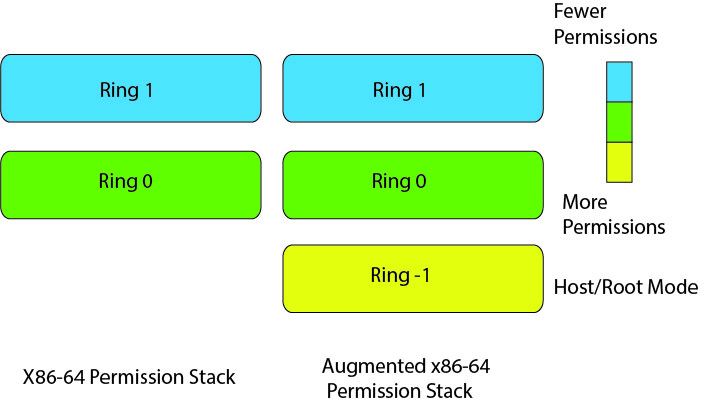
\includegraphics[width=\textwidth]{figures/AugmentedPerm.jpg}
	  \caption{Augmented x86-64 privilege Stack}
\end{figure}

\subsection{Virtualization}

Virtualization itself is not a new concept. It began in the 1960s with the IBM System 360 ~\cite{vleck_ibm_2010}. This system, like most others for the next nearly four decades, used the trap and emulate model. In this model a virtual machine (VM) will proceed unaltered until it reaches an instruction, which it cannot execute due to an insufficient privilege level ~\cite{popek_formal_1974}. The guest operating system then faults to the hypervisor which performs some set of instructions. This set of instructions will then perform an operation with an identical effect to the original instruction. 

In 1974 Popek and Goldberg ~\cite{popek_formal_1974} formalized the conditions, which were sufficient to allow a CPU architecture to support virtualization. To begin they define a Virtual Machine Monitor (VMM) as a piece of software which provides a programming environment which is ``essentially identical'' ~\cite{popek_formal_1974} to the machine being virtualized (fidelity), only causes a minor performance decrease (efficiency), and is in complete control of the resources (resource control or safety).

Popek and Goldberg then seperate CPU instructions into three different classifications.  Privileged instructions are those which will cause a fault if run in user mode (such as the Intel $cli$ ~\cite{_intel_2015} instruction), control sensitive instructions which change the configuration of resources in a system (the Intel $cli$ instruction also falls into this category),  and behavior sensitive instructions whose affects vary based on the configuration of resources (such as the $popd$ ~\cite{_intel_2015} instruction which varies based on privilege level).

With these requirements and definitions acting somewhat as axioms Popek and Goldberg give us two theorems ~\cite{popek_formal_1974}



 \begin{theorem}[Popek Theorem 1]
 \label{Popek I}
 {
 ``For any conventional third generation computer, a virtual machine monitor may be constructed if the set of sensitive instructions for that computer is a subset of the set of privileged instructions'' ~\cite{popek_formal_1974}
 }
 \end{theorem}


\begin{theorem}[Popek Theorem 2]
 \label{Popek II}
 {
 ``A conventional third generation computer is recursively virtualizable if it is virtualizeable and a VMM without any timing dependencies can be constructed for it.'' ~\cite{popek_formal_1974}
 }
 \end{theorem}



The proofs for these theorems can be found in the original work by Popek and Goldberg. The first theorem says that a VMM can only be constructed for an architecture if the sensitive instructions are a proper subset of the privileged instructions and the second says an architecture is not virtualizable if a VMM cannot be constructed for it.  

This model is not appropriate for x86 virtualization however as many of the x86 assembly instructions, such as $popd$~\cite{_intel_2015}(which pops an element off the floating point stack),  are sensitive but not privileged. This violates the conditions required for VMM construction of Popek's first theorem and by extension x86 cannot be virtualized via the trap and emulate method. 

In 1999 VMware patented their techniques for binary translation, which they introduced in 1998~\cite{rosenblum_vmwareas_1999}, allowing the x86 architecture to be virtualized.  In binary translation the hypervisor runs one ring below the guest OS (in Host/Root mode on x86-64).  The translator reads guest memory starting at the instruction pointer (eip/rip) and caches up to 12 instructions (fewer if a terminating instruction is reached) in a Translator Unit (TU). Unprivileged and non-sensitive instructions (such as $mov$ or $xor$) are translated IDENT (identically) with no changes made. 

Privileged and sensitive instructions however are translated producing Compile Code Fragments (CCF) using non-privileged instructions. Agesen et. al. ~\cite{agesen_evolution_2010} use the $cli$ instruction as an example. The $cli$ instruction clears the interrupt flag on the physical CPU. 
Since the guest VM cannot (and should not ) clear the interrupt flag on the physical CPU the interrupt flag is cleared on the VCPU ($vcpu.flag$) using the $and$ instruction. Once a TU is translated into a CCF it is then run on the CPU. 

This began the boom in x86 virtualization, which was shortly followed by the introduction of Xen in 2003~\cite{barham_xen_2003}, which introduced the paravirtualization method for x86 virtualization. In paravirtualization, like binary translation, the hypervisor runs at Ring 0, the guest OS runs at Ring 1, and user code runs at Ring 3.  Paravirtualization works by using a modified kernel, replacing instructions which will require hypervisor support such as those involving memory Managementment with hypercalls~\cite{barham_xen_2003}.  These hypercalls result in the hypervisor peforming some operations which result in the a state being presented to the VM which from its perspective appears that it has been performed on physical hardware rather than on a VM. This allows the guest to run without any modification to user space code much like trap and emulate and binary translation. This method, however, traditionally requires that a specific kernel be used, which greatly increases the time between versions and makes the virtual environment sensitive to OS changes. As of Linux version 3.0 however the introduction of Paravirt Ops into the Linux kernel has added native paravirtualization support removing this limitation~\cite{_understanding_????}. Due to the nature of paravirtualization we are limited in a practical but not theoretical sense to open source operating systems such as Linux~\cite{_Linux_archive} and BSD~\cite{mckusick_design_2004}.

The 64-bit line of x86 processors was introduced by AMD in 2003 and this line only had 2 level of privilege unlike the 4 in the 32 bit lines. The result was there was no longer room to run a hypervisor, guest OS, and user code each on their own privilege level. In 2006, Intel (VT-x ~\cite{neiger_intel_2006}) and AMD (AMD-V ~\cite{codenamed_pacifica_2005}) both added hardware virtualization to their x86 line of processors. Hardware virtualization adds another layer in the privilege stack below Ring 0 called the Host Mode and Root Mode for Intel and AMD respectively. These are colloquially, though not formally, referred to as Ring -1. A structure called a Virtual Machine Control Block (VMCB) is defined in hardware. This structure holds the list of all instructions to be intercepted. Certain instructions are required to fault by the hardware but others can be added to the VMCB by the hypervisor. This method allows the guest OS to run on Ring 0 of the hardware as it would normally expect to. The guest runs normally until it has to run an instruction which requires a fault (as defined in the VMCB). The instruction which caused the fault is then trapped and handled by the hypervisor. Any operating system can be virtualized in this manner, however it does require special hardware instructions (though those are now available on almost all Intel and AMD CPUs) and the shifts to the Host/Root mode are time consuming and need to be reduced to the smallest number possible to keep the process efficient.

Shortly after the advent of X86 hardware virtualization ~\cite{neiger_intel_2006}~\cite{codenamed_pacifica_2005} the hypervisor KVM (for Kernel Virtual Machine) was introduced by Kivity et al ~\cite{kivity_kvm:_2007} and was included as part of the main line Linux[18] kernel the same year. As part of the Linux kernel KVM is able to reduce some of the code base by incorporating certain aspects of the Linux kernel such as the scheduler in order to handle managing resources of virtual machines.  Throughout this experiment we will be using either Xen or KVM as appropriate. Due to the differing architectures of the two hypervisors there will be some approaches that will work with one and not the other. Where applicable we will comment on why one was chosen for a specific experiment over the other.





\subsection{X86-64 Memory Architecture}\label{x86mem}

Modern commodity CPUs use an architecture known as the Von Neumann Architecture ~\cite{von_neumann_first_1993}.  At the most basic level a computer based on the Von Neumann Architecture consists of a CPU which processed data and instructions, memory, mass storage, and input/output devices.  Due to limitations on the throughput between the different parts of a computer we encounter what's known as the Von Neumann Bottleneck~\cite{von_neumann_first_1993}.  Data on a CPU register is fast to access, RAM is slower, disk drives slower still, and network based storage the slowest available. 

To address this problem CPU cache was introduced. Cache is a small amount of extremely fast RAM which exists on the CPU in order to alleviate, but not eliminate, the Von Neumann Bottleneck.  In a modern X86-64 CPU there are three levels of cache: L1, L2, and L3. L1 is the smallest and fastest with L2 being slightly larger but slower and L3 being even larger and slower. 

On a modern CPU the process of accessing memory begins by checking the Translation Lookaside Buffer (TLB). The TLB is a small amount of cache which holdes virtual address translations in the form of Page Table Entries (PTEs). These entries (discussed further in section \ref{PageTable}) map virtual memory to physical memory. If the entry is in the TLB we have a TLB hit.  If this occurs we look to see if our physical address is in the L1 cache. If this is the case we have an L1 cache cit and the data is loaded into the CPU. If this is not the case we have an L1 cache miss. If this occurs we look to see if our physical address is in the L2 Cache. Again if it is we have an L2 Cache Hit and load our data to the CPU. If an L2 Cache Miss occurs we have to check the L3 Cache. Unlike the L1 and L2 Caches the L3 Cache is shared by all cores on a CPU. If our physical address is in the L3 cache we have an L3 cache hit and our data is given to the CPU. Otherwise it requires looking to see if the data is in DRAM. In the event of a TLB miss a walk of the page table is necessary (~\ref{PageTable}). 
\begin{figure}\label{X86Mem}
	  \centering
	  \includegraphics[width=\textwidth]{figures/X86MemoryHeirarch.jpg}
	  \caption{X86-64 Memory Heirarchy}
\end{figure}

Each of the steps described before contributes to our Average Memory Access Time (AMAT). The formula for computing AMAT is described in equation ~\ref{AMAT}. Where $H_i$ is the time per hit on the some memory element (e.g. Cache or the TLB), $AMP_i$ is the average penalty per miss on that element, and $M_i$ is that a miss will occur on that element. This is summed over all the elements of memory. 

\begin{equation}\label{AMAT}
	AMAT = \sum_{i=0}^{n}{H_i+AMP_i\times M_i}
\end{equation}

\subsection{Virtual Memory and Paging}\label{PageTable}

In a modern programming environment memory is abstracted so that each process sees its physical memory as one contiguous region.  This is a convenient abstraction made possible through virtual memory. In modern x86 and x86-64 virtual memory is provided through a system called paging. In paging memory is broken into segments called pages, which are typically 4kb though larger pages are supported up to 2MB and 1GB for 32-bit and 64-bit x86 respectively. A data structure called the page table is used to map virtual memory that the process sees to physical memory. In the x86 architecture this mapping is handled by hardware known as the Memory Management Unit (MMU). 

The x86-64 processor uses a 4 level paging system to translate virtual addresses to physical addresses when 4kb pages are used and a 48-bit address space. The levels are organized in a tree structure. The CR3 holds location of the page directory for the process. The first 16 bits are unused, next 36 bits are broken into four segments of 9-bits each. The first is called the Page Map Level 4 page (PML4), the next is called the Page Pointers Directory page (PDP), the next is called the Page Directory page (PD), and the final one is called the Page Table page (PT). The remaining 12 bits are for the page offset, which tells us where in the page the memory is located Fig ~\ref{VirtPaging}~\cite{_file:x86_2009}. 

\begin{figure}\label{VirtPaging}
	  \centering
	  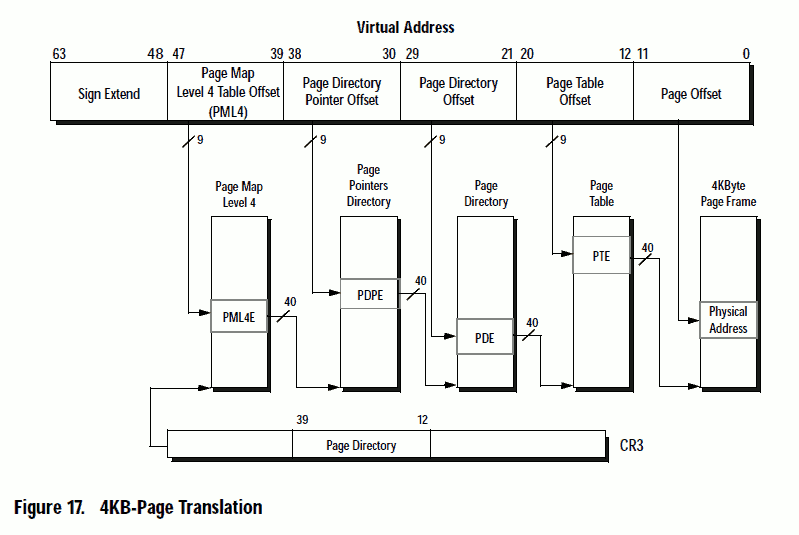
\includegraphics[width=\textwidth]{figures/Orion64BitTranslation.png}
	  \caption{Page Table in x86-64 ~\cite{OrionPaging} }
\end{figure}



\section{Xen}
Xen is a type-1 or ``bare metal'' hypervisor. This means that Xen runs directly on the physical hardware and is not itself hosted in another environment. This is in contrast to a type-2 hypervisor like VMWare Player which is hosted inside a Linux or Windows environment. Administration of Xen and its VMs is done via a special paravirtualized guest called the Dom0. All other guests in Xen can be either paravirtualized or hardware virtualized. For the remainder of this dissertation we will assume all DomU guests (those guests which are not Dom0) are hardware virtualized unless otherwise specified.

\subsection{Xen Virtual Memory Management}

As Xen supports two different types of virtualization it also supports three different kinds of virtual memory management. Traditionally software virtualization uses a shadow paging scheme ~\cite{barham_xen_2003} which keeps an additional ``shadow'' page table. This provides an additional layer of abstraction between the guests and the physical hardware. 

Since paravirtualized guests use hypercalls for sensitive instructions Xen is not required to keep a full shadow page table for its memory management, instead using a technique known as direct-paging. In direct paging guests invoke a hypercall which directly maps their page table entries from virtual memory to physical memory as opposed to the extra paging layer provided in shadow page tables~\cite{barham_xen_2003},  essentially moving control of memory management from the OS to the hypervisor. In this way ultimate control of memory management is transferred from the guest OS to the hypervisor. 


Since hardware virtualized (HVM) guests are not modified in the way that paravirtualized guests are, they do not have the option of this direct-paging technique and instead have the option of either hardware assisted paging (HAP) or shadow paging. HAP uses a technique called Second Level Address Translation (SLAT) Fig ~\ref{SLAT} which is included in Intel processors since the Nehelem line and AMD processors since the Barcelona line. Their technologies are called Extended Page Tables (EPT) and Rapid Virtualization Indexing (RVI) respectively. In SLAT the guest OS still maintains a logical page to physical page mapping (fig 2). However these physical pages are in pseudo pages and do not correspond directly to physical memory. Instead the hypervisor maintains the pseudo physical to machine page (or actual physical page) mapping.  


HVM guests also have the option of using a shadow page table (SPT) similar to that used in VMWare~\cite{rosenblum_vmwareas_1999}.  Like HAP shadow paging works by adding another layer of abstraction to paging. In this model the processes use the software page tables provided by the OS just like they would normally. When a guest OS tries to update a page a shadow page is allocated. This shadow page can be then altered with no constraints. When the page is ready to be moved into the regular page table (i.e. permanent changes have been accepted) references are updated such that they point to the new page rather than the original.

\begin{figure}\label{SLAT}
	  \centering
	  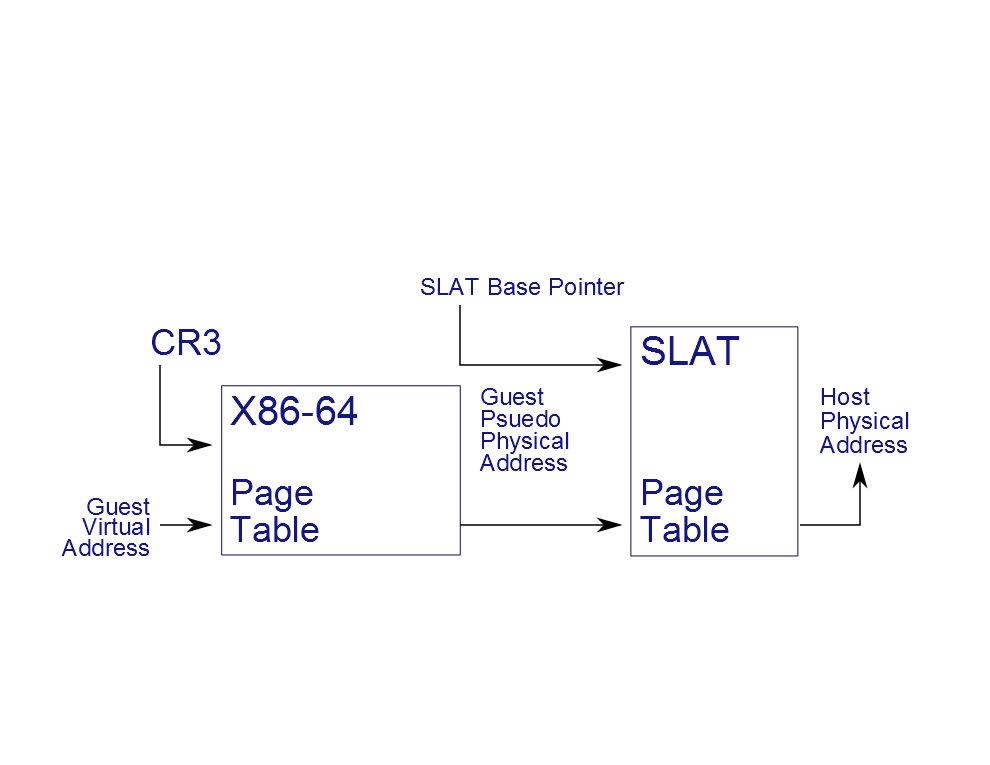
\includegraphics[width=\textwidth]{figures/BM_Graph1.png}
	  \caption{Diagram of Hardware Accelerated Paging using SLAT }
\end{figure}

\section{KVM}

Like Xen, KVM is a type-1 (i.e. Bare Metal) hypervisor. Unlike Xen, which is an independent hypervisor loading up a paravirtualized Linux VM as the administrative unit, KVM is itself integrated into the Linux kernel, which allows the use of a non-virtualized Linux environment for administration (as opposed to the paravirtualized Linux environment used in Xen). As a result of being part of the Linux kernel, KVM is able to use portions of the Linux kernel, for instance KVM uses the Completely Fair Scheduler ~\cite{pabla_completely_2009} used in the kernel to schedule CPU time for VMs. Other functions such as memory management are also done using the internal Linux mechanisms.  

\subsection{KVM Page Merging}

In version 2.6.2 of the Linux Kernel a scheme called Kernel Samepage Merging ~\cite{arcangeli_increasing_2009} was introduced. In this scheme pages which are identical among processes are merged in order to save memory. To accomplish this processes which may be candidates for merging register with the kernel. The kernel then scans the registered areas of virtual memory by taking the hash of those pages. Pages which have unique hashes are skipped for the remainder of the scan, while pages which have the same hashes are then checked byte by byte to ensure they are identical and avoid hash collision. Identical pages are then merged by first marking all page table entries where page occurs as unwriteable. Next all page table entries which refer to that page are updated so they point to only one instance of the page. The remaining unmerged copies of the merged page are then freed and a final direct memory comparison is made to ensure that the pages have not changed. These merged pages can only remain merged so long as the processes or VMs using them are only reading from them. To address this KVM uses a Copy-On-Write (COW) scheme. With this technique pages remain merged until one guests attempts to write to it. When that occurs a copy of the page is made for that guest and the remaining guests continue to use the merged page. 




\section{Virtual Machine Introspection}

Garfinkle and Rosenblum ~\cite{garfinkel_virtual_2003} introduced Virtual Machine Introspection (VMI) in 2003. In VMI the state of a running VM is interpreted by some external entity, usually either another VM or by the host system. To accomplish this memory is mapped or copied from the target VM to the VMI program. Memory is then interpreted to determine some portion of the internal state of the target VM. While the original work was used for intrusion detection a number of other applications have emerged in the years following. 

Memory outside of a given context has no intrinsic meaning,  only inside a given context or process does it have meaning. As such memory in a guest OS has no meaning outside of that guest. This problem is known as the semantic gap. The typical way to solve the problem ~\cite{garfinkel_virtual_2003} ~\cite{hay_forensics_2008} is to use a template approach for each individual OS. In this approach certain areas of memory are marked as being where certain structures in kernel memory are located.  That way a VMI agent can look for the relevant areas in memory and interpret them at run time.  The process of determining the location of these kernel structures can be time consuming, error prone, and must be repeated for each version of a running kernel. Work is being done to address the problem of the semantic gap and is addressed later in this dissertation. 

At its most fundamental level VMI represents a mapping of memory from the guest to an area outside of the guest (be it another VM as in the case of Xen or an administrative Linux OS as in the case of KVM). In this case we can study one method for VMI without losing generality. For our experiments we will use VMITools ~\cite{payne_vmitools_2014}. It is an open source framework to allow easy development of VMI applications, supports Linux and KVM, and has appeared in a number of works on VMI (though in some of these works it appeared under its former title XenAccess) ~\cite{dolan-gavitt_leveraging_2011, zhao_vrfps:_2009, lengyel_virtual_2012, weingartner_promox:_2009, marken_using_2014}.

\section{Virtual Machine Introspection Literature}

Gu et. al. ~\cite{gu_process_2011-1} introduced a scheme for active VMI. In this scheme for VMI a process is injected from the hypervisor to the guest VM. This process is hidden inside an innocuous process already running inside the VM. These processes are called the implanted process and the victim process respectively and are both chosen by the host administrator at runtime. When the victim process is scheduled to be run, the hypervisor captures the context switch. The implanted process the replaces the victim process. To accomplish this the relevant instruction pointers are changed as well as the relevant stack pointers etc. When the OS resumes to continue the context switch the implanted process is run in place of the victim process. Once the implanted process has completed or the hypervisor determines it is time to switch the context back the contexts are switched and the victim process runs is executed normally. 

In the initial experiments ltrace, a program to scan the libraries called by a process, is implemented as the implanted process. This allows them to implant ltrace into a running VM and are able to trace the library calls of selected processes. While this does accomplish some of the goals of conventional VMI it can also be unusable for applications such as digital forensics in which a VM must remain unaltered in any capacity in order to be of use in a courtroom setting. 

Dolann-Gavitt et al introduce a system called Virtuoso ~\cite{dolan-gavitt_virtuoso:_2011} which is aimed at bridging the semantic gap. The execution of Virtuoso is broken into three phases: The training phase, the analysis phase, and the runtime phase. 

In the training phase Virtuoso attempts to gain information about the guest. Inside the guest a program must be written to access the information desired. For instance if one were trying to write a VMI program to access the Process Identifiers (PIDs) then one would write an in guest program which would access the process IDs. This program would then be run repeatedly and each time it was run a syscall trace (such as with Linux strace) would be taken of that program.  After running this program repeatedly an extensive list of execution paths would be generated. Using this combination of execution paths the analysis phase can begin. 

The collection of syscall traces, while it does contain the necessary execution paths, also contains a great deal of extraneous noise. This is because the system trace follows the entire execution through the system not just the relevant information. Parts of the trace, which are known a priori to be unnecessary such as hardware interrupts or memory management, are thrown out immediately. Then a dynamic data slice ~\cite{agrawal_dynamic_1990} is then done. There slices are merged into a unified program which can be turned from an in guest program to an out-of-guest program. 

The translated code cannot be run directly on the host. So Virtuoso creates a runtime environment for the translated code. The run time environment is installed on the host machine and has the ability to run the translated code. This gives the code created by Virtuoso an appropriate context from which to access the VM resources (e.g. CPU registers or main memory) in a read-only manner.

While Virtuoso does make significant progress in bridging the semantic gap it does not change the fundamental nature of introspection. The tools generated by Virtuoso still simply read and interpret memory from the guest, which means that our study will still apply to virtuoso without having to directly address virtuoso. 


Like Virtuoso, Fu and Lin ~\cite{fu_bridging_2013} make an attempt at bridging the semantic gap and automatically generating VMI utilities.  The process begins with an untrusted target VM (called the product-VM) and a secure trusted VM (called the secure-VM). Three techniques are then used to extract information from the product VM. These are syscall execution context identification, redirectable data identification, and kernel data re-direction. 

The context being executed is identified using a stack to keep track of times iret  and int are called. Global kernel data is then identified using an adapted form of taint analysis. With the relevant information located and the contexts identified they are then able to redirect the kernel information between the product-VM and the secure-VM. This allows native system monitoring utilities to be run on the secure-VM as VMI targeting the product-VM unaltered. 

In their results many of the native Linux utilities such as lsmod ~\cite{kerrisk_lsmod8_2014} gave identical results as if they were inside the product-VM itself. However certain utilities like date ~\cite{mackenzie_date1_????} and ps~\cite{lankester_ps1_????} produce similar but not identical results. This was found to be due to the timing of the snapshots they were using for the analysis as certain programs are quite time sensitive. While this has approached an automatic bridge for the semantic gap this work is still reliant on semantic information about system calling conventions and can be altered if they are changed between kernels. This seems like a promising tool to use for VMI however as of this publication the source code has not yet been released for use by the public, so it will remain unstudied in this work. 


\subsection{Uses for Virtual Machine Introspection}
In this section we will discuss current uses for VMI especially as they related to information assurance and security. 

In Crawford and Peterson ~\cite{crawford_insider_2013} VMI is leveraged to address the insider threat problem.  The insider threat problem is the situation that occurs when current or past members of an organization have both malicious intent and legitimate access to a system or systems ~\cite{rushby_critical_1994}. To accomplish their goal they break their approach into four steps: Development of a taxonomy of malicious insider behavior, development of a taxonomy of VMI observables, malicious insider detection, and data validation. 

To develop a taxonomy they began by setting up a number of possible high-level uses cases. The activities identified in this taxonomy are printing activity, disabling defensive tools (e.g. anti virus), abusing removable media (e.g. putting sensitive information onto a flash drive), sudden change in employee behavior, use of remote access, and strange clipboard activity. Once they determine major uses cases they wish to look for they decompose each scenario into individual observable attacks and each attack is broken down into seven areas of analysis. These areas are the attacker (who is doing something or can do something), which tools are used, which vulnerabilities are used, what actions are taken in order to achieve the desired effect, which systems are targeted, what the result of this unauthorized attack is, and what the objective of that result is. Using this taxonomy they can break many insider threat problems into simple terms. 

The next step is to determine which parts of a system can be observed by VMI. The observables consist of ``registry information, hexadecimal patterns, and clipboard information.'' Each of the potential malicious activities is performed while the observables are being monitored by VMI. If those observable areas create signature patterns then they can be used to identify the insider threat actions from VMI. The relevant observables are provided in the work from Crawford and Peterson ~\cite{crawford_insider_2013}. 

The third step is essentially the experiment portion of the paper. During the experiment VMI is used as well as Windows event logs. VMI and Windows event logs are analyzed while certain potentially malicious operations described earlier were performed. The experiment recorded which actions set showed as being malicious and which ones did not. 

The final step is the analysis phase. For each attack in the scope of the research they perform it manually several times to determine if their tools developed from the third phase are capable of detecting it. Their results showed that they were able to detect 18 different types of insider attacks. They report a high false positive rate though they don't give the specific rate of either detection or false positives. The authors indicate that while this work shows potential more work needs to be done on determining which observables correlate to which observables can indicate attacks in order to increase the accuracy of their detection. 

Harrison et al ~\cite{harrison_constructing_2012} have proposed using VMI combined with the related yet distinct field of Forensic Memory Analysis (FMA). Harrison's goal is to put together an entirely out-of-band passive sensor to monitor for malicious software such as kernel rootkits. Like all current VMI approaches FMA is adversely affected by the semantic gap. In order to address this situation a file system was built using FUSE~\cite{rajgarhia_performance_2010}, which translated the page table such that the memory of the VM was able to be read as one contiguous ``file''. The volatility framework for FMA is then used in order to analyze the contents of the memory. A rule learning algorithm called IREP++ ~\cite{dain_irep_2004} is used as a classifier in order determine if any intrusions are made into the system (such as kernel rootkits) were made and the results are logged into a postreSQL database. This is an interesting approach to side-stepping rather than attempting to directly solve the semantic gap. Volatility however like many VMI approaches still relies on a priori knowledge of the location of data structures inside the kernel which may leave this approach vulnerable to attacks which manipulate those structures. 

Hay and Nance ~\cite{hay_circumventing_2012} developed a method for using VMI to read the plaintext for encrypted data with the VIX tool suite~\cite{hay_forensics_2008}.  While direct attacks on modern cryptographic systems such as AES is generally computationally intractable three basic facts are noted: Before being encrypted cipher text exists in an unencrypted form, after being decrypted cipher text exists in an unencrypted form, and encryption requires that somewhere on the system cryptographic keys exist. To take advantage of the first two it is a simple matter of observing the state of VM while the plaintext is in memory.  The third requires two steps; recover the key while it exists in memory and use that key as to recover the plaintext using the appropriate decryption algorithm. This use of VMI is an instance of security software which has great use for law enforcement and intelligence agencies as well as great potential to be misused as well.

\section{Information Leakage and Side Channel Attacks}

In this section we discuss the current state of research into information leakage and side channel attacks.

\subsection{Side Channel Attacks}
While a number of side-channel attacks have been explored in the past~\cite{yu_approach_2013,ristenpart_hey_2009, zhang_cross-vm_2012} a formal model of the information leakage due to these attacks was first introduced by Demme et al ~\cite{demme2012side}. Demme introduces the Side-channel Vulnerability Factor (SVF) in order to determine exactly how vulnerable a certain cross-channel attack makes a system. 

The SFV begins with an oracle, which contains the truth about the execution of the victim. The side-channel produces the information that an attacker is able to measure. An example of an oracle could be number of accesses to a certain page and the side-channel could be the average power consumption on the host. A perfect side-channel would be able to trace the oracle trace directly. The SVF also requires a distance metric. The distance metric could vary from problem to problem. For instance if the data were represented by vectors the Euclidean or Manhattan distances could be used. 


Next they establish a similarity matrix for both the oracle and side-channel traces. These similarity matrices are necessary since oracle and side-channel are by their very nature measuring different things (such as pages accesses versus cache access time).  

Next they establish a similarity matrix for both the oracle and side-channel traces. These similarity matrices are necessary since oracle and side-channel are by their very nature measuring different things (such as pages accesses versus cache access time).  The similarity matrix M is defined as being of length $S$ and size $|S|^2$.  Each element of $M$ is defined as 




\begin{equation}\label{eqn:simMatrix}
M(i,j) =  
		\begin{cases}
			D(S_i, S_j) & if \ i  >  j \\
			0 & otherwise \\
		  \end{cases}
\end{equation}

where $D$ is our distance function.  This creates a triangular matrix with no diagonal. The matrices are compared elementwise and the Pearson correlation coefficient between the two is computed. The further from 0 the Pearson Correlation Coefficient is the more information is leaked through a side channel. A coefficient of 1 will mean the channel is perfectly transparent and a coefficient of 0 will mean that the channel is totally opaque. 

This SFV will be able to provide us with a measure to tell how our different approaches to information leakage will be relative to each other. As well as a measure of how much information leaks from VMI relative to other types of information.

\subsection{Determining Co-Residency} 
Ristenpart et al ~\cite{ristenpart_hey_2009} introduced a scheme for determining co-residence by measuring the load on the cache. In their paper they did a variant on the cache-probe technique which relies on the architecture of the x86 cache. It begins by allocating a buffer $B$ of size $b$ bytes, where $s$ is the size of the cache line.  Their initial attack is broken into three pieces

\begin{enumerate}
	\item Prime: Read $B$ at $s$ byte offsets. (Ensuring that $B$ is in cache)
	\item Trigger: Wait until the number of CPU cycles passed jumps by some large value (to determine if the VM has been interrupted by the Xen credit scheduler)
	\item Probe: Measure how long it takes to read $B$.
\end{enumerate}

In step 3 $B$ is accessed in pseudorandom order in order to prevent the hardware pre-fetcher from hiding the latency. These latencies correlate strongly with use of cache during the trigger step. However due to Xen s scheduling algorithm this is not quite enough to measure the cache latency. For that they expand the prime-probe attack even further to the following.

\begin{enumerate}
	\item Allocate $B$ contiguous bytes.
	\item Sleep briefly (to build up credits with Xen's scheduler)
	\item Prime: Read all of $B$ to make sure it's fully cached
	\item Trigger: Busy loop until the number of CPU cycles jumps by a large value
	\item Probe: Measure how long it takes to read $B$
\end{enumerate}

Through this load measurement and comparison to VMs running known services they are able to determine which VMs are co-resident. 

Zhang et al ~\cite{zhang_cross-vm_2012} put forth another scheme for determining co-residency of VMs on the Amazon EC2 cloud ~\cite{_aws_EC2_2014} by measuring the load on the cache. In this attack we consider two entities $U$ and $V$ each of which share a common cache. Then a similar prime-probe method as above is used though it is modified to function as follows

\begin{enumerate}
	\item Prime - $U$ fills a cache set by reading a region from its own memory
	\item Idle - $U$ waits for a specified interval during which the cache is used by $V$
	\item Probe - $U$ times the reading of the same cache set in order to learn of $V$`s activities
\end{enumerate}


In their initial trials the VM represented by $U$ attempted to determine if $V$ was co-resident by running one prime-probe trial and averaging the time across all cache sets. If this time was below a certain threshold a foe-absent classification was issued and if it was below that threshold a foe-present classification was issued. This proved to be extremely unreliable for two primary reasons: The Xen scheduler balances load by shifting VMs to different cores which may not share physical caches and because friendly VM activity on other cores , especially IO activity, will cause activity in the Dom0 which will introduce significant noise into the cache. In order to deal with this high level of noise a multi-probe classifier was implemented. In this classifier they looked at the results of 2000 prime-probe trials and noticed a pattern appearing to be two overlapping normal distributions. They then use these statistics to determine the classification. 

In Owens and Wang ~\cite{owens_non-interactive_2011} a scheme using the memory de-duplication techniques provided by commodity hypervisors (specifically ESXi ~\cite{chaubal_architecture_2008} in this case). They begin by assuming that an attacker can instantiate VMs in the same environment as the targeted VM and that the attackers has root control over any VMs it instantiates. Further they assume the standard 4kb pages size. To begin their procedure they first determine which pages are unique to a specific OS version and are present in all versions of that OS. They must also determine which of those pages are relevant to their analysis, for example a memory dump of Windows XP SP3 contains 59,238 pages of zeros~\cite{owens_non-interactive_2011} These are not useful to the analysis. They are then able to determine which pages are signature pages for each OS. 

At this point they take advantage of the de-duplication mechanism in ESXi. When ESXi writes a non de-duplicated page a simple write is performed. However when writing to a de-duplicated page a copy is made of that page and then it can be written to. The memory allocation and copy of the new page takes a measurable level of overhead. While there is overhead from the copy it can also be easily confused with the computational overhead from reading a page which has been swapped out having not been used recently. To handle this a read operation is performed on the signature page immediately before attempting an OS fingerprinting operation. They are then able to plot the timing results and can demonstrate which OS is being run on the host. 

Xiao et al ~\cite{xiao_security_2013} explored the implications of memory de-duplication on security in a more general sense by putting together both a reliable attack using this technique and a reliable defense against similar techniques. For their offensive approach Xiao shows that one can transmit data between two co-located VMs using the memory de-duplication. 

They begin with two co-located VMs with a hypervisor which uses memory de-duplication. Each VM creates a number of identical pages. This can be easily accomplished by reading an identical file into memory. Then the sender encodes the information which it wants to transmit to the receiver. It does so by writing to certain pages and not to others. The sender and the receiver then sleep for some amount of time to allow the pages to be merged by the hypervisor's memory de-duplication mechanism. The receiver then writes to each of the pages and times the amount of time it takes to make these changes. Because of the Copy-On-Write(COW) nature of these systems it takes slightly longer to write to a de-duplicated pages as it makes a copy before writing to it. In this way memory can be encoded into bits. A page which has been merged representing a 0 and a page which has not representing a 1. So if both VMs allocate 8 pages in this manner and wishes to transmit 10011001 the sender would alter pages 1,4, 5, and 8 so they would not merge. 

In addition to transmission they were also able to determine that one was in a virtualized environment using the artifacts of memory de-duplication. A file is read into memory and then all pages in memory are written to and the write access times are recorded. Then the file is read in its entirety into two different memory locations. Since every page of the file has an exact duplicate in memory the hypervisor’s de-duplication mechanism (if present and virtualized) is likely to merge the pages after an appropriate amount of time. Then one of the identical pages can be written to, if the environment is virtualized with memory de-duplication then the write access time will be significantly higher than the original write access times due to COW. 


Yarom and Falkner ~\cite{yarom2013flush+} expanded upon the Prime-Probe attacks described earlier with their Flush+Probe attack which they use to read cryptographic keys from a VM. In this attack we again consider two entities $U$ and $V$ which are co-located on the same socket though not necessarily the same core. It follows that $U$ and $V$ would then share the same L3 cache since they are co-located on the same socket. 





As a defensive mechanism agaisnt these attacks Xiao suggests a kernel runtime integrity scheme.  There several hypervisor based mechanisms for determining the presence of kernel rootkits running in guests ~\cite{butler_windows_2005}~\cite{hoglund_*real*_1999}. These all require extensive knowledge of the kernel in order to bridge the semantic gap. Xiao proposes examining the kernel for the sections of data, such as the syscall table, which are meant to be read-only. Inside the kernel binary read only data is designated by the .rodata section. This data is copied and read by a C program inside which holds an exact copy of the read only kernel data in memory. 

A statistic gathered by Linux called the Proportional Set Size (PSS) is then used in order to determine whether kernel integrity has been threatened. The PSS value is the number of unique pages and the weighted number of the duplicated pages a process has. For instance a process with 100 unique pages and 100 duplicated pages would have a PSS of 150 ~\cite{xiao_security_2013}. This value is stored in the file /proc/\$pid/smaps. A simple shell script can then determine if the PSS value has increased significantly to determine if kernel integrity has been violated. 

These side-channels are directly applicable to determining whether or not a VM is being monitored by VMI. Linux uses a technique called Kernel Same Page Merging (KSM) to reduce memory commitment from processes in a manner similar to how ESXi de-duplicates pages for VMs. The KVM hypervisor treats all VMs as if they are Linux processes. As a result it is possible that identical pages between a VM and some Linux process can be merged thus causing a measurable delay when these pages are written to. If the VMI program happens to hold a page identical to one in a guest VM then it's possible that the VMI process can be detected through this delay. 

Zhang et al ~\cite{zhang_cross-vm_2012} introduced a scheme for reading cryptographic keys used by another VM sharing the same physical hardware and hypervisor. A similar prime-probe technique to was used, but this time specifically used on the instruction cache (icache) as opposed to the data cache (dcache). It does so with the standard icache technique introduced by Aciicmez ~\cite{aciiamez_yet_2007}. A icache line is loaded with nops and then filled again with nops and the time difference between the two is noted. Further steps are needed however, as information from another VM is being sought the Xen scheduler has to be taken into account. To handle this interprocessor interrupts (IPIs) are used. In symmetric multiprocessing (SMP) systems processors are allowed to interrupt each other or even themselves through an IPI. To make sure the attacking VCPU has precedence another VCPU (called the interrupting VCPU or IVCPU) runs in a continual loop sending IPIs to the attacking VCPU.

This attack searches for instructions which are a square, a multiply, or a modulus-reduce instruction. In order to do so they use multiclass support vector machine[68] to pick out when these instructions are being used. While this is fairly good at picking out instructions the SVM is subject to the hardware and software noise introduced by the system (things such as TLB misses, or context switches.) To handle this hidden markov models ~\cite{bishop_pattern_2006} are used to filter the noise. This allows them to determine the cryptographic key in as little as 40,000-50,000 brute force attempts. While this may seem like a great deal we keep in mind that 50,000 brute force attempts will take less than 1s on commodity hardware making this a reasonably effective attack. 

These previous works have been directed almost entirely at exploring side-channel attacks aimed at the hypervisor layer. Bates et al ~\cite{bates_detecting_2012} take a lower level approach and investigate whether co-residency of one or more VMs on a hypervisor can be determined via active traffic analysis techniques. They begin by assuming that they are on a normal cloud instance such as EC2~\cite{_aws_EC2_2014} that has been patched against previous co-residency attacks ~\cite{zhang_homealone:_2011}~\cite{ristenpart_hey_2009}. 

\begin{figure}\label{BatesNetworkThing}
	  \centering
	  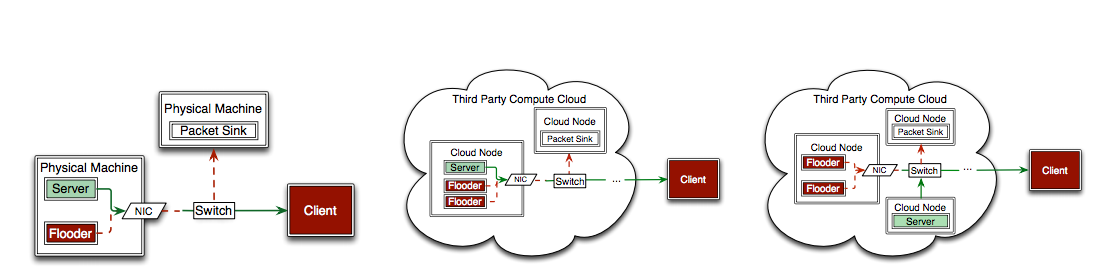
\includegraphics[width=\textwidth]{figures/batesNetwork.png}
	  \caption{Topologies used in active traffic colocation test from Bates et. al. ~\cite{bates_detecting_2012}
	  (left) local test system 	(center) successful co-location   (right) failed co-location }
\end{figure}



Their attack then creates a large number of instances on that cloud service, which they term flooders. Each flooder announces its presence to an external machine called the client. Another instance created in the cloud is called the server. Upon receiving a signal from the server the client sends signals out to the flooders, at which point the flooders begin to send outbound traffic on their machines physical interface to a packet sink which is not the client. This outbound traffic causes a delay in the server flow. 

These delays in server flow form a watermark in the signal from the client and the server. The network flow between the client and server can be given by $T$ and divided into $n$ segments of $t_i$. Watermarks of this kind require two different levels of packet delay to encode their signal represented by $\pm d$. Since negative delays are not possible in this environment they take no delay to represent $-d$ and a delay to represent $+d$. Using this scheme they are able to encode bit values using $-d$ as a 0 and $+d$ as a 1. 

Due to the nature of virtualization and network traffic in general a certain amount of noise can affect the signal. These can come from sources such as network congestion or hypervisor scheduling (as described above in the Xen Credit Scheduler for instance.) When the client receives the signal a Kolmogorov-Smirnov (KS)~\cite{pettitt_kolmogorov-smirnov_1977} test is done for independence. If a signal is embedded in the traffic flow it will demonstrate a different discrete distribution from one without a signal. With the KS test they are able to determine a signal's independence with a 95\% confidence. 

This attack is interesting in that it operates at the hardware layer rather than at the hypervisor layer. It is possible that VMI targeted at the network stack of a VM (such as the VIX ifconfig ~\cite{hay_forensics_2008} ) could cause a change in the delay, which could be detected in the traffic. However this delay is unlikely to be substantial or consistent enough to useful to detect information leakage from VMI.

\subsection{Detection and Defense Against Attacks}

Martin et al ~\cite{martin2012timewarp} introduced a scheme to protect against micro-architectural attacks by obscuring the way the rdtsc instruction works. Micro-architectural attacks such as the cache timing attacks described above ~\cite{zhang_cross-vm_2012,ristenpart_hey_2009,zhang_homealone:_2011} rely on precise timing of micro-architectural events in order to gather their information. Martin proposes a scheme by which they add two delays to the rtdsc counter. One, called the real offset, delays the execution of the rdtsc instruction. The other, called the apparent offset, which adds a random delay to the end of the rdtsc instruction. These delays can turned off in the OS so that system critical portions of the OS such as the scheduler are not interfered with.  While this can be quite effective against certain types of attacks like those listed above it can be easily worked around if an attacker can gain kernel access (for example through a kernel module) and gives their malicious process rights to use the unaltered scheduler. While this may pose a challenge for some side-channel attacks their threat model differs from ours significantly enough that it poses no hindrance.

\section{VMI and Kernel Attack Papers}

Bahram et al ~\cite{bahram_dksm:_2010} introduced a scheme to subvert VMI through Direct Kernel Structure Manipulation (DKSM) also known as direct kernel object manipulation (DKOM). In this scheme the data structures which store information, such as the list of processes, are manipulated in such a way as to attack the semantic gap. 

The way most VMI implementations are implemented a template based scheme is used to solve the problem of the semantic gap. For each kernel known addresses, such as the start of the task list, are fetched on the assumption that their address and composition are invariant. The DKSM attacks this assumption. 

Bahram et al use three different designs for their DKSM attack: a syntax based manipulation, a semantic based manipulation, and a hybrid scheme. The syntax based attacks take advantage of the fact that some fields in the kernel data structures are not used by the OS. An unused field is removed thus changing the template used by the VMI implementation and rendering its output inaccurate.  In the semantic based scheme fields in some data structure of the same length and similar type are swapped so that their order is reversed. This has the same effect rendering the template used by the VMI implementation useless. The hybrid scheme is a combination of the two where fields are removed and rearranged. 

The implementations of these schemes tested are the direct scheme, and the shadow scheme. A third, the return scheme, is discussed but not implemented. The direct scheme manipulates the structures directly using a loadable kernel module. This method had the advantage of being comparably simple to implement but is easily detectable by VMI tools which choose to measure the kernel integrity making it somewhat impractical. 

The shadow scheme begins by taking advantage of the fact that on commodity x86 processors data and code have separate caches specifically the icache and the dcache. As there is a data cache and an instruction cache there is also a data and instruction Translation Lookaside Buffer (DTLB and ITLB respectively) which will be the target of this attack. 

The ITLB is invalidated at some address (pte) causing that page entry to be ejected from the ITLB. A page, located at address pte, which contains the instructions for the DKSM attack called a ``shadow page'', then replaces the page that was ejected. The global bit on the shadow page is marked to prevent it from being forced out of the ITLB due to TLB pressure from context switches. At the end of the DKSM code in the shadow page is a jmp instruction which jumps to the location of the previously invalidated code. This has two functions: First it loads the page into the icache and the ITLB and secondly it returns control flow back to the original code. This scheme is far stealthier than the direct scheme described above, however it is also far more complicated to implement. Both implementations above are reliant on a modified version of the hypervisor (specifically QEMU/KVM ~\cite{bellard_qemu_2005} in this case) in order to trace memory to learn which fields of a kernel structure are accessed by which functions. This makes these attacks impractical outside of a laboratory environment and the first to take in improving them would be to rectify this short-coming by setting up a way to analyze kernel structure access internally. Further this paper only explored the ``spatial'' aspect of introspection. That where the structures are in memory and ignored the time based aspect of introspection which takes a finite amount of time to create its view and thus is potentially vulnerable to timing based attacks~\cite{bahram_dksm:_2010}. 


% include statement for Chapter 2 (really, the first actual chapter)
\chapteruaf{The Plan}

\section{Motivation and Goals}

	With the increase in the use of VMI (drop your citations in here) in research settings as well as the migration of VMI to the commercial sphere ~\cite{_vmware_2014} the study of the security of this technique has taken on paramount importance. With the use of VMI to extract cryptographic keys from live memory ~\cite{hay_circumventing_2012} the dangers of misuse of VMI have become apparent. TODO (REWORD). 

	In this dissertation we have two goals

	\begin{enumerate}
	\item To detect the use of VMI on the guest VM from within the VM. 
	\item To , in some way, impair the use of VMI on the guest VM. 
	\end{enumerate} 

	For the detection of VMI we aim to determine if VMI is being run on the guest in any capacity. Our threshold for successful detection is a simple yes or no answer to the question “Can the guest detect that it is being monitored by VMI?” Any results which exceed this threshold will also be taken as confirmation of detection of VMI.

For the goal of impairing or subverting VMI we take as the threshold for success any  results which will affect the availability or integrity of the VMI agent being tested. 


\section{Threat Model}
	We begin defining the Trusted Computing Base (TCB) as the set of all hardware and software which is essential to the security of a computer system ~\cite{rushby_critical_1994}. Vulnerabilities in the TCB will be considered vunerabilities in the whole of the system. Components outside the TCB should not be able to elevate privileges than they are granted by the OS or hypervisor. 

	For the following experiments we will assume that the hypervisor as well as all associated interfaces such as libvirt or xencntrl are part of the TCB. All VMI agents will also be assumed to be part of the TCB. The guest VM will be outside of the TCB and therefore all malicious code must be executed on the guest VM. We further assume that the malicious VM is isolated from all other VMs. 

	The attacker on the malicious VM will be assumed to have root access to the VM and therefore will be allowed to install malicious kernel modules as well as run malicious user code. 

\section{Experimental Setup}

	The hosts in our experiments will use version 4.2 of Xen~\cite{barham_xen_2003} and version 3.2.0 of KVM ~\cite{kivity_kvm:_2007}along with version 1.6.2 of QEMU~\cite{bellard_qemu_2005} (the userspace component to KVM). Guests are Ubuntu Server VMs with Linux kernel version 3.11.0-12-generic~\cite{_Linux_archive}. Guests are allocated 1GB of RAM and 1VCPU. Unless otherwise stated all VMs are clones of the original VM created. 

	For experiments concerning the detection of VMI a simple system will be used where one guest VM is run on a physical host system (fig 2.1). 

	\begin{figure}\label{ExpApp}
	  \centering
	  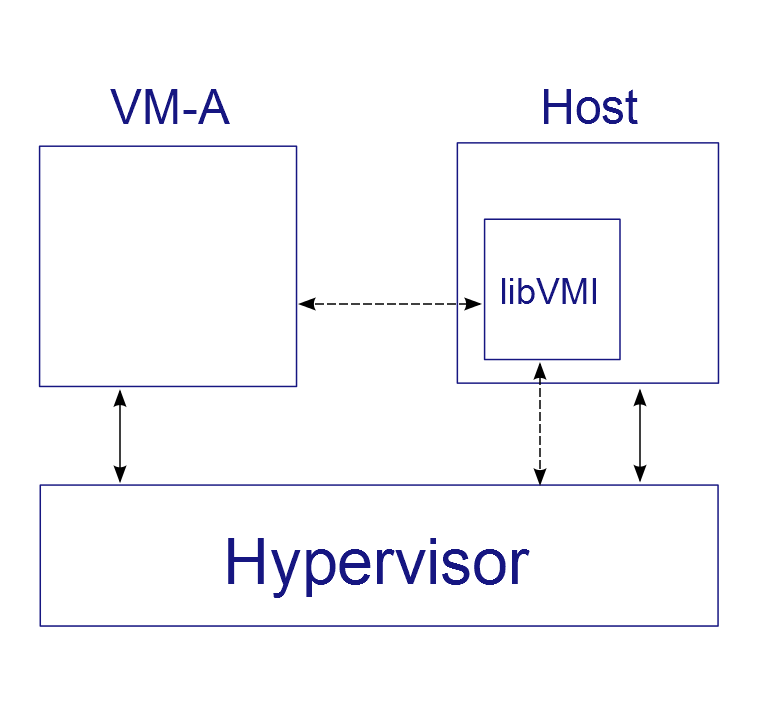
\includegraphics[width=\textwidth]{figures/BM_graph3_cropped.png}
	  \caption{Experimental Setup}
	\end{figure}

\section{VMI Agents}
For the detection of VMI all experiments will be using VMITools~\cite{payne_vmitools_2014}. Since the primary means of doing VMI is to copy a page from memory then interpret it [cite a few], any toolsuite which does this can be used for this experiment without the loss of generality. There will be three VMI programs used for these experiments; map-addr, process-list, and module-list. 

The map-addr program simply maps an address from the guests memory to the memory of the VMI agent. The process-list command maps the processes currently running on a VM. In Linux the list of running processes is stored in the task-list (cite sched.h). The task list is a doubly linked list where each node in the list represents a process being handled by the OS. The process-list program begins by mapping the head node of the task list from the guest to the VMI agent. The first task struct is then decoded. The desired information , such as pids and process names, is displayed to the user and the location of the next task in the list is recorded. The next node in the task list is processed in the same way. This continues until the list comes back to the head of the task list, indicating that the entire list has been traversed. 

% \begin{pseudocode}{process-list}{ Domain}
% 	current_task=Domain.task\_list\_head
% 	\REPEAT 

% 		adr=adr.nextTask
% 		map nextTaskStruct to host
% 		translate nextTaskStruct
		
% 	\UNTIL current\_task.addr=task\_list\_head.addr
% \end{pseudocode}


The module list works in much the same way. 


\section{Experiments}
In this dissertation we propose five experiments. Four experiments will be used to detect VMI and the last will be an attempt to subvert VMI by gaining control of the host through the VMI channel. 

For our first experiment we wish to analyze data produced by the Linux utility Sysstat~\cite{godard_sysstat_2010}. Sysstat measures over 200 (TODO Figure out the right amount) fields used by Linux such as page faults per second, context switches per second, and percentage of swap space used. Since the host, guest, and VMI agent all use the same physical resources it is possible that the patterns can emerge in those numbers which can identify the use of VMI on the guest. 

For our second experiment we propose to analyze the time it takes to map and unmap a page in memory. With main memory and the page table being shared between VMs,  it's possible that the use of a VMI agent on the guest will cause a distinguishable difference in the time taken to do the mapping and unmapping of a page.

Our third experiment is similar to the first experiment in that in memory timing is used to determine if a guest is being monitored by VMI. In this case it's the use of the CPU cache. If they are on the same CPU a guest and a VMI agent will share the same L3 cache. If they are on the same core they will share the same L2 and L1 cache as well. For our experiment we propose measuring how long it takes to write an element in memory. Between each measurement we flush all three caches. We hypothesize there will be a small dip in the time required to access memory after it has been flushed from cache if a VMI agent has been accessing memory in that program. (TODO FIX to make specific about the page being monitored) 


Our fourth experiment takes advantage of the fact that KVM uses several features of the Linux kernel. In this case the scheduler and the KSM mechanism. KVM uses the Linux scheduler, in this case the Completely Fair Scheduler (CFS) ~\cite{pabla_completely_2009}, to manage VMs essentially as Linux processes. As a result of being treated as Linux processes, KVM VMs are subject to memory de-duplication using KSM. We hypothesize that the memory de-duplication can be measured as in (TODO cite the previous two) if a VMI agent copies a 

\section{On Timing}

In this chapter we will be discussing the analysis of a number of different timings. For these timings we used the C++11 chrono object~\cite{_chrono_2014}. The C++ chrono object offers a high-resolution timer, the resolution of which is dependent on the system. In Linux the high-resolution timer offers nanosecond resolution.  In order to determine the resolution and any computational overhead for the chrono object we take a sample inside the guest VM. In this sample we simply run take two time measurements one after the other and log the difference between them. We take 1,000,000 measurements like this and plot them Figure RawTiming. What we see is that while we have nanosecond resolution there is a significant amount of overhead involved in the start of a timing measurement. In order to compensate for this we take the minimum value of our measurements and subtract it from all subsequent measurements. 

\begin{figure}\label{RawTiming}
	  \centering
	  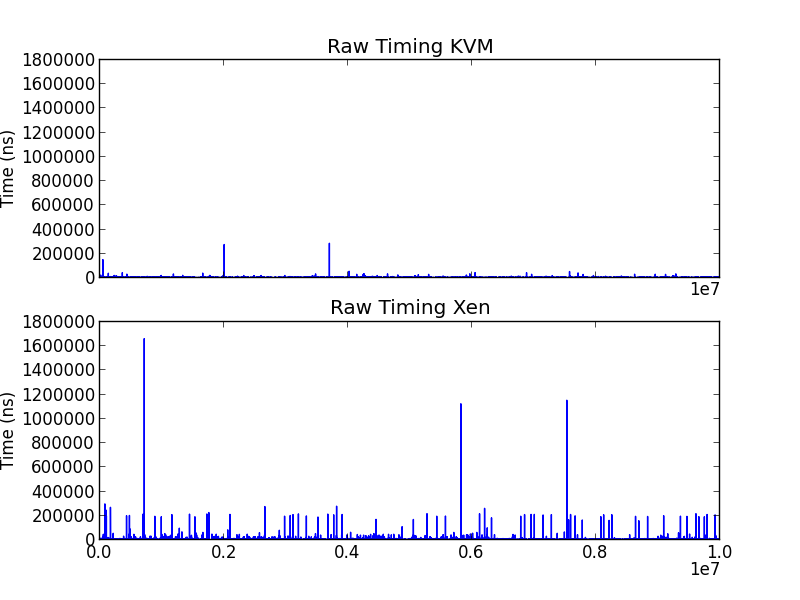
\includegraphics[width=\textwidth]{figures/RawTimingXenandKVM.png}
	  \caption{Raw Timing for Xen and KVM}
\end{figure}


The minimum value is quite close in both KVM and Xen at 549 ns and 539 ns respectively. These measurements represent the bare minimum amount of time it takes to perform a timing measurement so we can subtract it as overhead on subsequent measurements.  

%% adding these here so they're ready for page 3 of the ToC, and page 2 of the LoF. YMMV. Move as needed.

% include statement for Chapter 3
\chapteruaf{Common Analysis Tools}
\section{Introduction}
In this chapter we will be discussing a number of statistical terms and methods which will be common to the remainder of this dissertation. 

\section{Definitions and Terms}
We begin our discussion by defining the terms population and sample. A population is the complete set of data that have one property in common that is the subject of some statistical analysis. A sample is a subset selected from a larger population~\cite{devore_probability_2011}. For example we might consider a population as all people over 1.8m tall and a sample could be 1,000 randomly chosen people over 1.8m tall. 

Next let us consider a sample $X$ drawn from some population. Further let us define an individual element in $X$ as $x_i$ where $ \{x_1, x_2, ....., x_{n-1}, x_n \} \in X$. Next we assume that each $x_i$ has a probability of occurrence of $p_i$. Further we assume that all values in $X$ are independent and identically distributed (iid). That is, no element in X depends on another and all elements are pulled from the same distribution.  We define the mean of $X$ as~\cite{wackerly_mathematical_2007} 

 \begin{equation}\label{mean}
 	\mu=\frac{\sum_{i=1}^{n} x_i}{n}
 \end{equation} 

This represents the ``average'' value of the dataset. We further define the standard deviation of the dataset ~\cite{wackerly_mathematical_2007} as 

\begin{equation}\label{sigma}
	\sigma = \sqrt{\sum_{i=1}^{n}p_i(x_i-\mu)^2}
\end{equation}

The standard deviation gives a measure of how dispersed the sample is from the average. Finally we define the define the variance of $X$ which is simply $\sigma^2$ and gives a measure of how spread out the sample is. 

\section{Hypothesis Testing}
In this test we will be using statistical hypothesis testing in order to analyze our data. Hypothesis testing is the process of using statistical test to determine whether a hypothesis about some model is false. We begin by defining the null hypothesis $H_0$ as some claim we initially assume to be true ~\cite{devore_probability_2011}. The alternate hypothesis $H_a$ is the claim we assume to be true if we reject $H_0$. 

When discussing hypothesis testing we will be comparing two random samples. The first sample is $X$ where  $X_i$ has a probability of  $p_{xi}$ and $\{x_1,x_2,...,x_{n_x}-1 , x_{n_x}\} \in X$ . The second sample is $Y$ where  $Y_i$ has a probability of  $p_{yi}$ and $\{y_1,y_2,...,y_{n_y}-1 , y_{n_y}\} \in Y$ .

Using an appropriate statistical test (discussed in sections ~\ref{sec:ttest} and ~\ref{sec:mannWhitney}) we will be able to compute our test statistic. A test statistic a the result of a function of our data which gives us one number upon which we can base our rejection of $H_0$. Given the test statistic we can then compute our $p$-value. The $p$-value is the probability ``calculated assuming $H_0$ is true of obtaining a test statistic at least as contradictory to $H_0$ as the value actually computed''~\cite{devore_probability_2011}. That is, a $p$-value gives us the probability that our test statistic would have been produced if $H_0$ were true. The smaller the $p$-value the more the data contradicts $H_0$. Note this is not the same as saying the $p$-value is the probability that $H_0$ is true nor is it the error associated with our test. Next we have our critical region which is the set of values for which we reject $H_0$. If our $p$-value falls in our critical region we reject $H_0$.

When we discuss hypothesis testing we must also discuss the types of errors associated with it. A type \Romannum{1} error is when one asserts that $H_0$ is true when it is in fact false. This is also called a false positive. A type \Romannum{2} error is when the null is false but is not rejected. This is also called a false negative. 

\subsection{Welch's t-test}\label{sec:ttest}

The first hypothesis which will be used is Welch's t-test\cite{welch_generalization_1947}. In Welch's $t$-test we look at the two populations and calculate a $t$-statistic. This is more robust for our purposes than the more common student $t$-test as it does not assume both samples $X$ and $Y$ have the same variance. Based on this statistic we can determine whether or not to reject the null hypothesis.  

We next compute the t-statistic for the two populations $X$ and $Y$ via the following formula:

	 \begin{equation}\label{t-stat}
		t = \frac{  \mu_x - \mu_y }{ \frac{\sigma_{x}^2}{n_x} + \frac{\sigma_{y}^2}{n_y}   }
	 \end{equation}

Now that we have the $t$-statistic we can begin to compute the $p$-value. First however we need to determine the degrees of freedom $\nu$ for our test. For each of our random samples $X$ and $Y$ the degrees of freedom are given by $\nu_x = n_x -1$ and $\nu_y = n_y-1$. We can then approximate the degrees of freedom for Welch's $t$-test using the Welch-Satterthwaite equation ~\cite{satterthwaite1946approximate,welch_generalization_1947}

	\begin{equation}\label{tTestDegrees}
		\nu \approx \frac{ (\frac{\sigma_{x}^2}{n_{x}^2}+\frac{\sigma_{y}^2}{n_{y}^2})^2 }{\frac{\sigma_{x}^4}{n_{x}^2 \nu_x}+\frac{\sigma_{y}^4}{n_{y}^2 \nu_y}}
	\end{equation}

With the degrees of freedom for the test we can compute finally compute the $p$-value by using the probability density function (pdf) for student's $t$-distribution. 

\begin{equation}\label{tTestPDF}
	f(t)=\frac{\Gamma(\frac{\nu+1}{2})}{\sqrt{\nu}\Gamma(\frac{\nu}{2})}(1+\frac{t^2}{2})^{\frac{-\nu+1}{2}}
\end{equation}

where 

\begin{equation}\label{Gamma}
	\Gamma(a) = \int_{0}^{\infty} x^{a-1}e^{x}dx
\end{equation}

We now obtain the $p$-value by integrating the pdf of student's $t$-distribution from $t$ to $\infty$. 

\begin{equation}\label{pvalStudentTest}
	p=\int_{t}^{\infty}f(t)dt 
\end{equation}

With the p-value in hand we can determine whether or not to reject the null hypothesis by selecting a critical value. If the p-value is smaller than that critical value then we can reject the null hypothesis that the two distributions share a mean.  For all t-tests in this dissertation we will assume a critical value of 0.001. We will be performing all of our t-tests with the scipy library~\cite{jones_scipy:_2001}. It should be noted that many of the p-values obtained in this dissertation are 0. For a finite dataset it is impossible to obtain a p-value of 0, this instead a limitation of IEEE floating point arithmetic and should be taken as less than  . While these values may initially appear suspicious it should be noted they can easily be verified by performing the integral manually (or rather with a numerically using a different function in scipy~\cite{jones_scipy:_2001}).  It can also be intuitively verified if one looks at the student-t distribution for one degree of freedom (fig ~\ref{TDist}).  We see that as x increases P(x) goes to 0.  

\begin{figure}\label{TDist}
	  \centering
	  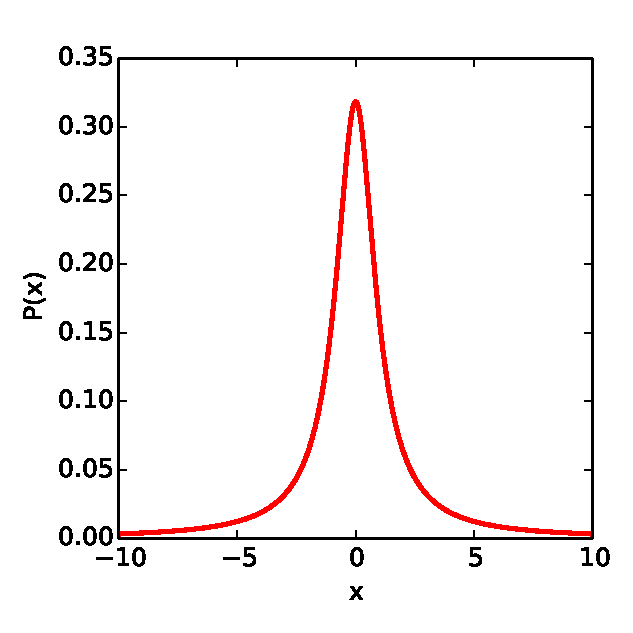
\includegraphics[width=3in]{figures/T_distribution_1df.eps}
	  \caption{t-distribution for one degree of freedom}
\end{figure}

\subsection{Mann-Whitney U Test}\label{sec:mannWhitney}

The Mann Whitney U-test ~\cite{wackerly_mathematical_2007} , also called the Wilcoxon rank-sum test, is a hypothesis test which tests the null hypothesis that one sample has tends to have larger values than another. We begin the Mann Whitney U-test using the same populations, means, and standard deviations as in Welch's t-test. Then we check to see whether or not the following four assumptions are satisfied. 

\begin{enumerate}
	\item $X$ and $Y$ are independent of each other
	\item All observations are ordinal (i.e. it can be distinguished that one observation is greater than another) 
	\item Under the null hypothesis both groups are equal
	\item Under the alternate hypothesis the probability of an observation from one population exceeding an observation from the other is not 0.5. 
\end{enumerate}

In order to perform the test we compute the $U$ statistic.  There are two methods for computing the $U$ statistic: one for small data sets (less than 20 elements) and one for larger data sets.  As all of the datasets used in this are on the order of $10^6$ elements we will only be discussing the latter.

The first step is to rank all the observations. The smallest observation is assigned the rank 1, the next smallest value is assigned the rank 2, and so on.  Ties are equal to the midpoint of the assigned rankings. So in the set $\{2,4,4,7\}$ the ranks $\{1, 2.5, 2.5, 4\}$ would be assigned. 

The next step is to sum the ranks of all observations taken from $X$ and call it $R_1$.  The sum of the ranks from observations taken from $Y$ is given by $R_2$. We can then then compute the $U$ statistics 

\begin{equation}\label{U1}
	U_1=n_1 n_2 + \frac{n_1(n_1+1)}{2} - R_1
\end{equation}

\begin{equation}\label{U2}
	U_2=n_1 n_2 + \frac{n_2(n_2+1)}{2} - R_2
\end{equation}

The smaller of $U_1$and $U_2$ is chosen for computing the p-value which are obtained through a table of critical values. As with the t-test we will be using the scipy implementation ~\cite{jones_scipy:_2001} for our Mann Whitney U-tests. 

\section{Mutual Information}

Mutual information is a quantity which measures the amount of certainty gained about a population $X$ when measuring some random variable $Y$.  In particular let $Y\in {0,1}$ represent whether or not the VM is monitored by some VMI agent and let $X\in \mathbb{R}^n $represent the measured data from a given experiment.  The mutual information   then specifies how many bits of information are gained about $Y$ when sampling the random variable $X$.  Given a joint probability distribution $P(Y=y,X=x)$  the mutual information is given by 

\begin{equation}\label{MutInformEq}
	I(Y:X) = \sum_{x\in X}\sum_{y\in Y} p(y,x)lg(\frac{p(y,x)}{p(x)p(y)})
\end{equation}

To estimate the mutual information, we use the implementation provided by scikit-learn~\cite{pedregosa_scikit-learn:_2011-1} where $X$ is approximated by histograms over a large number of sample measurements. Mutual information will allow us to determine how much many samples are needed in order to make a classification between two samples. 

\chapteruaf{Sysstat Experiment}
\section{Introduction and Motivation}
In our first chapter investigating methods of detecting VMI we first ask ``What are the shared resources we need to investigate?'' and ``How can we get the information we need from these shared resources?'' Since all physical hardware is shared between the host and the guest we have an abundance to choose from such as memory, CPU, disk, and the network. We can get this information directly from the OS itself as a fair amount of information is recorded by the OS. In this experiment we will take that information provided by the OS and analyze it to determine if it can yield information about the use of VMI on that guest. 


\section{Sysstat}

Modern OSs log a large amount of information for performance and monitoring purposes such as the page fault rate, CPU frequency, and disk IO rates. In the Linux OS a program called Sysstat ~\cite{godard_sysstat_2010} makes this information easily available to the user. In this experiment we attempt to analyze the data produced by Sysstat in order to determine if a VM is being monitored by a VMI agent. We hope the use of an extant tool like sysstat will allow easy monitoring of this field by a system administrator and will require minimal setup on their part. 

\section{Experiment}

We begin our experiment with the same apparatus as described in section ~\ref{Apparatus}. For our first step we synchronize the clocks on the host and guest. We do this using the NTP protocol ~\cite{mills_internet_1991} available in Linux. Synchronizing the clock on the host and guest allows us to compare measurements taken by Sysstat on the guest to times when a VMI agent was used by the host.


On the guest Sysstat is run to gather all data it's capable of gathering. The interval is set to 1s as it is the smallest measurement Sysstat can take. One hour of data was taken. The command used to gather the data is 

%TODO FIX LATER
%Specifically centering
\begin{center}\label{SAR}
\begin{verbatim}
	sar -A 1 3600
\end{verbatim}
\end{center}

On the host we run a script called \textit{collectData.py} (Appendix I). This script runs a VMI program specified for a user and at a time interval also specified by the user. For our experiment we run the VMI programs \textit{process-list}, \textit{module-list}, and \textit{map-addr}. We do our measurements at intervals of 100s, 50s, 25s, 10s, and 5s. Each time a measurement is made the time stamp is noted.

\section{PreProcessing}

The data produced by Sysstat is stored in a difficult to read binary format. In order to convert this into an easily readable format we use the program sadf~\cite{godard2010sysstat} which converts the binary data to a more useful format (a .csv file in our case). This file however is still somewhat difficult to read for the average csv reader as the data is not uniformly formatted.  Upon inspection of this field (insert here) is uniformly 0 in all of our measurements which allows us to exclude the data from our analysis. Further complicating matters is that the majority of the measurements taken by Sysstat are not of the same unit. This poses two problems: you cannot directly compare measurements of different units and that different measurements are often of different scales. For instance you cannot compare amperes and meters as one measures electrical current and one measures distance. Further an every day measurement of current may be on the order of $10^{-3}A$ but measurements of distance might be on the order of $1m$. So while a change of $10^3$ might be insignificant for a measurement of distance it might be very significant for measurement of current. To address this problem a common technique called Z-score is used. To compute the Z score of a data set we first split the data set into features. A feature is a type of measurement in our data set such as page faults per second. Since our data is conveniently divided into fields we will use each field as one feature. For each feature we compute the mean ($\mu$) and the standard deviation ($\sigma$). Then for each datum $x$ in the feature we compute and replace it with $Z$ ~\ref{ZScore}.


\begin{equation}\label{ZScore}
	Z = \frac{x-\mu}{\sigma}
\end{equation}


This however will not work when $\sigma$ is 0 which will occur when there is no variation inthe data at all. When this occurred we were able to inspect the features which were uniformly which allowed us to remove the feature entirely. 

After the features were preprocessed we matched them with the times that the VM was monitored by VMI as noted by \textit{collectData.py}. We compare the time stamps taken by sysstat to the ones taken by \textit{collectData.py}. Data points which are within $0.5s$ of the time noted by the VMI program are marked as monitored by VMI and denoted with a 1. Other points are marked as unmonitored which is denoted by a 0. 

After processing the data we still had more than 150 features available each with 3600 measurements which can be quite a large dataset when using machine learning algorithms which can be quite slow. To do this we employ feature selection.


\section{Analysis}
\subsection{Information Gains}
Suppose we have a dataset $X$ with $x_i$ samples of class $i$ and $m$ classes total (in our case two for monitored and unmonitored). The amount of information needed to classify a sample is given by 

\begin{equation}\label{InfoGain}
	I(x_1,...,x_m)=-\sum_{i=1}^{m}\frac{x_i}{x}log_2 \frac{x_i}{x}
\end{equation}

Now let us denote a feature by $F$. A feature $F$ is made up of $\nu$ subsets $\{x_1,x_2,...,x_\nu \}$ where $x_j$ is the subset of $F$ with the value $f_\nu$. Now we let $x_j$ contain $x_{ij}$ samples of class $i$. We can then compute the entropy of the feature with equation ~\ref{Entropy} 

\begin{equation}\label{Entropy}
	E(F) = \sum_{j=1}^{\nu} \frac{x_{1j}+x_{2j}+...+x_{mj}}{s}I(x_1,...,x_m)
\end{equation}

The information gain is then computed as 

\begin{equation}\label{Gain}
	Gain(F)=I(x_1,...,x_m)-E(F)
\end{equation}

Using the information gain we are able to select the features which contribute the most information to classifying the datum. 

\subsection{Weka}
For our classifications rather than using the \textit{Scikit-learn} as we did with our previous chapters we will be using the machine learning tool Weka ~\cite{hall2009weka}. Weka was chosen as it has a graphical interface which lets us switch between machine learning methods for rapid prototyping. 
% include statement for Chapter 4
\chapteruaf{Using Page Allocation Timings to Detect VMI}\label{MMapChap}

\section{Motivation}\label{MMapChap-Intro}
In this chapter we discuss a simple statistical analysis of the time taken to map a page in main memory. When we look at resources shared between the Host and the Guest one of the most obvious ones is main memory. In the x86-64 processor main memory by the Memory Management Unit (MMU), which uses a process called paging to control which data and instructions are held in main memory. 

When a VMI program is used on a guest memory is mapped from the memory space of the guest to the memory space of the host (which, for brevity, we will refer to as guest-space and host-space respectively). We believe this mapping from guest-space to host-space will affect which pages are in memory to a degree that is measurable in the time required to map a page in memory.  


\section{Experimental Design}\label{MMapChap-ExpDesign}

For our initial experiment we aim to determine whether or not a guest VM can detect that it is being monitored by a VMI process. We begin by using the same experimental hardware described in chapter 2.  For our experimental setup we use a KVM and a Xen host. Each host runs a single VM of Ubuntu 14.04 as described in chapter II.  

On the host the VMI agent was run continuously. We did three trials: one where the process-list command was run, one where the module-list command was run, and one where the map-addr command was run. In each case the VMI program is continually run on the guest VM. 


On the guest side a probe is set up. This probe uses the C++11 chrono object~\cite{_chrono_2014} which gives us nanosecond resolution. For each iteration the time stamp is recorded, a page is mapped and unmapped from memory using the mmap function~\cite{_mmap2_2014}, and then the timestamp is again recorded. The difference between the second time stamp and the first time stamp are taken and this result is recorded as the time taken to map and unmap a page. As mentioned earlier however a small correction is made and the overhead time in the previous section is subtracted from the result to give our final result.  A control sample where no VMI agent is being run on the guest is also taken. 


\begin{enumerate}\label{MMapAlg}
	\item Mark Timestamp $t_0$
	\item map page in memory
	\item unmap page in memory
	\item Mark Timestamp $t_1$
	\item Record $t_1$-$t_0$
\end{enumerate}

\section{Results and Analysis}\label{MMapChap-Results}

The first step of our analysis is to compare the histograms of the control data with data here VMI is used.  It can be seen immediately (figs ~\ref{XenMMapHist1} and ~\ref{KVMMMapHist1}) that not only are the samples with VMI different from the control sample but they are also different f
rom each other as well. One should note that these histograms are zoomed in to give a better insight into the data. There are still small pockets of data after the 10,000ms bin but these are so small as to be not evident in the histograms.  The next step is to determine whether or not these datasets are statistically different from the data in the control sample. To do this we use two statistical tests, which determine whether or not two populations share the same mean. The first is Welch's t-test ~\cite{welch_generalization_1947} which determines whether the mean of two populations is the same. The second is the Mann Whitney U-test which again measures whether the two means of the population are the same.


	\begin{figure}[p!]\label{XenMMapHist1}
	  \centering
	  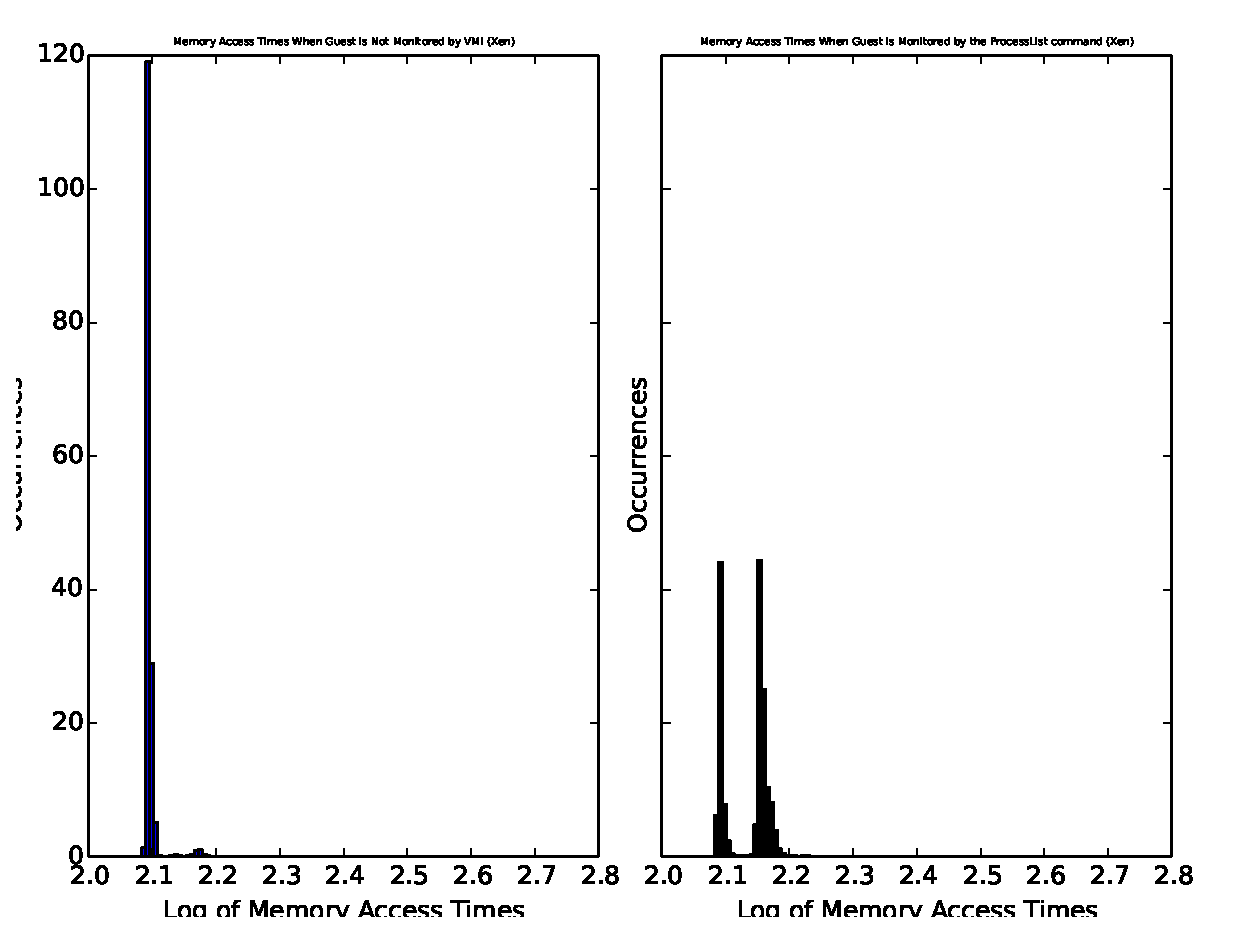
\includegraphics[width=\textwidth]{figures/XenNoVMIVsProcList.eps}
	  \caption{Histograms of the log of mmap time when a Xen VM is not observed by VMI (left) and observed by the process-list command (right)}
	\end{figure}


	\begin{figure}[p!]\label{KVMMMapHist1}
	  \centering
	  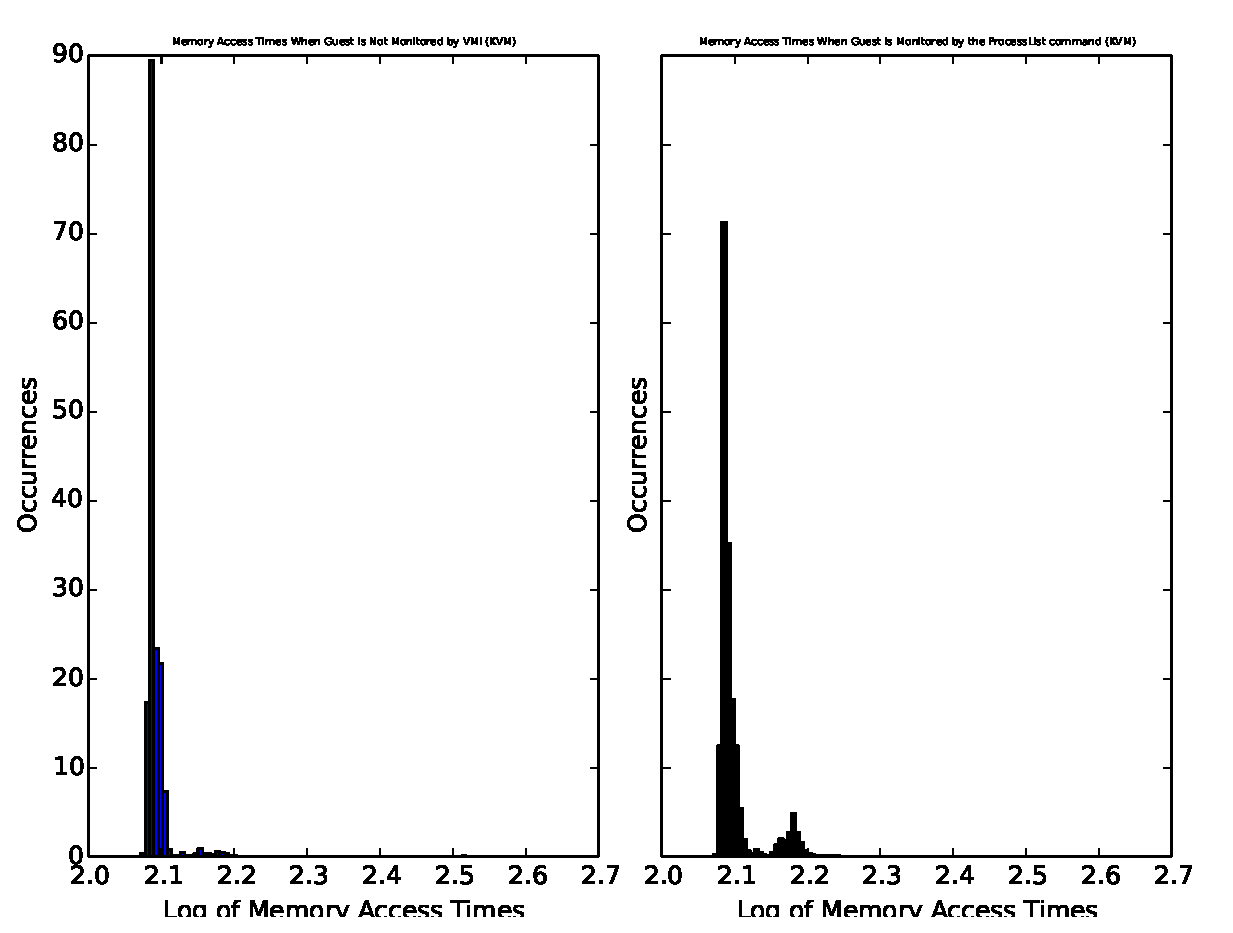
\includegraphics[width=\textwidth]{figures/KVMMMApTestNoVMIvsProcList.eps}
	  \caption{Histograms of the log of mmap time when a KVM VM is not observed by VMI (left) and observed by the process-list command (right)}
	\end{figure}

In both cases we begin with the null hypothesis that the mean of a sample not being monitored by VMI is the same as the mean of a sample which was being monitored by some form of VMI. The results of these tests are shown in table ~\ref{TStatsMMap1}. 
As we can see the results of the likelihood of the means of the two populations being is extremely low. It should be noted here that while all of the p-values are 0 this is strictly speaking not possible for finite populations. Instead this is a limitation of IEEE floating point arithmetic and a value of 0 should be taken as a value of less than $10^{-6}$.

	\begin{table}[p!]
		\centering
		\begin{tabular}{| c | c | c | c |}
			\hline
			Hypervisor & mapPage & modList & procList  \\ \hline
			Xen & -4361 & -5678 & -1691  \\  \hline
			KVM & -903 & -1000 & -632  \\ \hline
		\end{tabular}
		\label{TStatsMMap1}
		\caption{T stats for Xen and KVM compared to the null hypothesis that no VMI is being used}
	\end{table}

	\begin{table}[p!]
		\centering
		\begin{tabular}{| c | c | c | c |}
			\hline
			Hypervisor & mapPage & modList & procList  \\ \hline
			Xen & $3.73x10^{8}$ & $8.71x10^{8}$ & $7.43x10^{8}$  \\  \hline
			KVM & $8.34x10^{8}$ & $1.02x10^{9}$ & $3.26x10^{8}$ \\  \hline
		\end{tabular}
		\label{MannWhitneyMMap1}
		\caption{U stats for Xen and KVM compared to the null hypothesis that no VMI is being used}
	\end{table}



The next question to arise is this are these patterns unique to VMI or can theya be reproduced by other means? To answer this we first consider which factors can impact time taken to map a page are page faults and cache misses~\cite{bryant_computer_2003}.  At the scale of time being dealt with in this experiment cache misses will likely not be a significant factor given that they tend to operate in the 100ns range. As a result we will instead focus on page faults. 

\section{Elimination Experiments}

For this portion of the experiment we will test whether a VM with more memory will cause similar patterns in the time it takes to map a page  to those caused when a VM is being monitored by a VMI agent. We begin this portion of the experiment by cloning our initial VM but changing configuration so the VM has 4GB of RAM instead of the one it had earlier. The probe process as described in section ~\ref{MMapChap-ExpDesign} is repeated. The results are compared to the null hypothesis that the target VM is being monitored by the process-list program. 


We can see that these histograms are distinctly different (fig ~\cite{KVMMMapVS4Gig}. We then compare the two samples using the Mann-Whitney U test and the t-test we can see that the p-values are well outside our critical range and thus we reject the null hypothesis that two samples are the same. 

	\begin{figure}[p!]\label{KVMMMapVS4Gig}
	  \centering
	  \includegraphics[width=\textwidth]{figures/ProcListVS4GigKVM.eps}
	  \caption{Histograms of the log of mmap time when a KVM VM observed by the process-list command(left) and when a KVM VM has 4GB of RAM (right)} 
	\end{figure}

Next we test whether a VM which has more VCPUs can be confused with the signal of a VMI agent. We begin this portion of the experiment by cloning our initial VM but changing configuration so the VM has 3 VCPUs  instead of the one it had earlier. The probe process described in ~\ref{MMapChap-ExpDesign} is repeated. We again make the null hypothesis that the target VM is being monitored by the process-list program. 

We can see that these histograms are distinctly different (fig ~\ref{KVMMMapVS43VCPU}). We then compare the two samples using the Mann-Whitney U test and the t-test we can see that the p-values are well outside our critical range and thus we reject the null hypothesis that two samples are the same.


	\begin{figure}[p!]\label{KVMMMapVS43VCPU}
	  \centering
	  \includegraphics[width=\textwidth]{figures/ProcListVS3CPUKVM.eps}
	  \caption{Histograms of the log of mmap time when a KVM VM observed by the process-list command(left) and when a KVM VM has 3VCPUs (right)}
	\end{figure}


	\begin{table}[p!]\label{TableCPURAM}
		\centering
		\begin{tabular}{| c | c | c |}
			\hline
			 ``fill something in here '' & Mann-Whitney  & t-test  \\ \hline
			3VCPU & $ 1.184x10^{7}$ & $174.0$  \\  \hline
			4GB RAM & $1.373x10^{7} $ & $147.1$   \\  \hline
		\end{tabular}
		\label{MannWhitneyMMap1}
		\caption{U stat and t stat for populations taken when the VM had 4GB of RAM or 3VCPUs compared to the null hypothesis that they were being monitored by a VMI agent.}
	\end{table}

We next attempt to determine whether or not the number of VMs running on the same host will produce a signal similar to the one produced by a VM being monitored by a VMI agent. We begin our experiment by making three identical clones of our initial VM (now called VM-A) which will be labeled VM-B, VM-C, and VM-D as shown in figure ~\ref{Fig4VMTest}. We run an experiment initially where only VMs A and B are running. The probe described in section ~\ref{MMapChap-ExpDesign} was run on VM-A while VM-B was idle. We repeat this process with VMs A-C running and again with VMs A-D running.  We then compare each of these samples taken to the samples when a VM is being monitored by VMI (insert fig). 
	
	\begin{figure}[p!]\label{Fig4VMTest}
	  \centering
	  \includegraphics[width=\textwidth]{figures/BM_graph2_cropped.png}
	  \caption{Diagram of multi VM experiment} 
	\end{figure}


An interesting phenomenon occurs when one looks at the means of each of the samples taken in this experiment. When we compare the sample taken with two VMs running to our control sample there is a substantial decrease in the mean time taken to map a page. This average time then increases when a third and fourth VM are added (fig ~\ref{Fig4VMTest}).

	\begin{figure}[p!]\label{Fig4VMTest}
		\centering
		\includegraphics[width=\textwidth]{figures/mmapTimesOverVMsIdentical.png}
		\caption{Average MMap vs How many VMs are present}
	\end{figure}

What is causing this decrease in average mmap timing? We hypothesize that since the VMs are clones of each other the time merging of identical memory among the VMs has decreased the average memory access time by decreasing the number of cache misses since kernel data strutures are more likely to be in cache when accessed by another VM with an identical kernel. To test this hypothesis we repeat this exeriment however instead of cloning VM-A for VMs B-D we use CentOS Linux. If our hypothesis is correct we will now see a decrease in the average time taken to map a page when VM-C is added. We can see this occurred in fig ~\ref{Fig4VMTestCentOS} Thus indicating that our hypothesis was correct.

\begin{figure}[p!]\label{Fig4VMTestCentOS}
		\centering
		\includegraphics[width=\textwidth]{figures/CentOSTimesVsVMKVMANDXEN.png}
		\caption{Average MMap vs How many VMs are present when VMs B-D are CentOS VMs}
	\end{figure}

 

\section{Conclusion}
In this chapter we successfully introduced a method for detecting VMI as well as distinguishing between which VMI agent was used. It was also distinguish between multiple VMs being used as well as different levels of resource allocation. While it is impossible to exhaustively test all scenarios we consider this experiment to be a success as it did detect VMI. However it was not without its limitations. The VMI agent had to be run continuously without break on the VM in order for this method to be successful. This means that while successful in a technical sense it isn't especially realistic. 

\chapteruaf{Using Cache Timings to Detect VMI}

\section{Motivation and Introduction}
In this chapter we discuss a statistical analysis of the time taken to write to a page after it has been forcibly ejected from cache. When we look at resources shared between a host and guest one of the obvious ones is the CPU cache.  When a VMI agent fetches memory from a guest VM it ends up in the CPU cache. The question is can this caching be measured by the guest VM?  We hypothesize that there will be a measurable decrease in the time taken to access a page at intervals where VMI has been performed on the VM. In order to make this more general we aim our experiment at the L3 cache specifically. While each core has its own L1 and L2 caches, the L3 cache is shared across all the cores on a CPU.  This will mean we will be able to tell if a VM has been monitored by VMI agent regardless of which core it's on. 


\section{Experiment}

We begin this experiment with the same physical setup described in chapter II.   Since this experiment will be specifically measuring the L3 cache timings we don't need to pin the hypervisor and VM to the same VCPU. This experiment is broken into two portions: the monitoring portion and the host portion. 

When a VMI agent is used on a VM the memory being analyzed is copied or mapped from the VM to the VMI agent. This will move this data into the CPU cache of the CPU  on which the VMI agent is being run. Suppose the VMI agent were co-located on the same CPU as the VM being monitored. This would mean that the VMI agent would be able to fetch the memory from cache rather than having to go out to main memory.This would cause a significant decrease in the time taken to fetch the data.  Now suppose that the process inside the target VM which is being monitored by the VMI agent flushes cache lines which its memory occupies. This should cause a measurable increase in the amount of time required to access the data which has been evicted. 

For this experiment a process (the monitoring process) will be run on the guest VM. This process begins by allocating a page of memory and seeding it using the mersenne twister algorithm~\cite{matsumoto_mersenne_1998}. The mersenne twister is chosen to increase the probability that page will be distinct from all other pages in memory. This is to ensure when the data is evicted from cache it will not be inadvertently loaded by other processes, which have the same data in memory. 


\begin{algorithm}\label{CacheProbe}
\end{algorithm}


The monitoring process will then take one time stamp using the chrono object described in section 4.2, write to a random element in the page, then take another time stamp, and record the difference between the timestamps. The monitoring process then flushes the cache using the X86 $clf$ instruction ~\cite{_intel_2014}. This instruction flushes a cacheline from all levels of cache on the CPU. Since instruction only flushes a cache line the page is simply iterated through until all cache lines are flushed. This process is then repeated 1,000,000 times. 

On the host side the VMI agent will fetch the memory from that process and page. The VMI agent was run at regular intervals during the experiment. Trials were performed where the VMI agent was run every 50$\mu s$ , 100 $\mu s$ , 200 $\mu s$, 1ms, 10ms, and 100ms. Trials were also performed where the target VM was not monitored by a VMI agent. 

\section{Analysis}

The result were plotted and it was expected that noticeable drops in the time taken to write to a page would be present at regular intervals where the VMI agent had mapped the guest data. From Fig Y we can see that these drops memory access time are not present. Why is this the case? According to Hennesy and Patterson ~\cite{hennessy_computer_2012} say that a cache miss has takes approximately 25ns. This is a full order of magnitude less than the overhead taken for our timing measurements. Can anything be salvaged from these results? 

When one takes a histogram of the results 3 one can see that the histograms are slightly different. To determine whether or not this difference is significant we employ the t-test ~\cite{welch_generalization_1947} on pairs of datasets. The t-test gives us a measure of the difference between two samples called the t-statistic. By integrating the student-t distribution from the t-statistic to the p-value can be determined. The p-value gives us the probability that the t-statistic could be obtained under the null hypothesis that both samples are drawn from the same population. 

For the initial set of tests the t-test is run between pairs of populations with the control population being unmonitored by VMI and the variable population being monitored by VMI at some regular interval. Table 1 shows the results. In all the tests performed the p-value was less than $10^{−6}$. A $p$-value this small indicates that we can reject the null hypothesis that both samples were drawn from the same population. As a result we can take conclude that VMI has been detected by this probe.
In these tests 1,000,000 samples were used. This is an extremely large sample size and may not be useful for real time applications. The question now becomes can the sample size be reduced and still give acceptable results? Further how far can the sample be reduced and produce acceptable results? 


\begin{table}\label{TTestsCacheTiming}

  \begin{tabular}{| c | c | c | c | c | c |}
    \hline
    hypervisor & $50\mu s$ & $100\mu s$ & $200 \mu s$ & $1ms$ & $10ms$ \\ \hline
    Xen & -9.196 & -44.15 & -18.40 & -4.742 & -32.22 \\ \hline 
    Xen 100 Samples & -40.66 & -29.62 & -32.62 & -28.71 & -34.00 \\ \hline
    KVM & -12.25 & -12.33 & -11.29 & -12.25 & -11.36  \\ \hline
    KVM 100 Samples & -32.63 & -34.63 & -3.159 & -33.29 & -13.43  \\ \hline 
  \end{tabular}
  \caption{T Tests for Xen and KVM vs the null hypothesis that the no VMI has been used}
\end{table} 


\begin{table}\label{MannWhitneyCacheTiming}

  \begin{tabular}{| c | c | c | c | c | c |}
    \hline
    hypervisor & $50\mu s$ & $100\mu s$ & $200 \mu s$ & $1ms$ & $10ms$ \\ \hline
    Xen & -9.196 & -44.15 & -18.40 & -4.742 & -32.22 \\ \hline 
    Xen 100 Samples & -40.66 & -29.62 & -32.62 & -28.71 & -34.00 \\ \hline
    KVM & -12.25 & -12.33 & -11.29 & -12.25 & -11.36  \\ \hline
    KVM 100 Samples & -32.63 & -34.63 & -3.159 & -33.29 & -13.43  \\ \hline
  \end{tabular}
  \caption{T Tests for Xen and KVM vs the null hypothesis that the no VMI has been used}
\end{table}


\begin{center}\label{InfoGainsCacheAttack}
	\begin{table}
	  	\begin{tabular}{| c | c | c | c | c | c |}
		    \hline
		    hypervisor & $50\mu s$ & $100\mu s$ & $200 \mu s$ & $1ms$ & $10ms$ \\ \hline
		    Xen & 0.061 & 0.060 & 0.060 & 0.060 & 0.064 \\ \hline 
		    KVM & 0.070 & 0.069 & -0.071 & 0.070 & 0.073 \\ \hline   
		\end{tabular}
		\caption{Information Gain Results for Xen and KVM in bits}
  \end{table}
\end{center}


To determine this, we model the experiment as two random variables and considering the mutual information between them as discussed in chapter III. The results of the mutual information between the timing data and the presence or absence of VMI are shown in table 2, and demonstrate that by taking timing measurements, we gain as much as 0.08 bits of certainty about the VMI hypothesis. 


This indicates that the number of samples required can be reduced significantly from the original 1,000,000. We reduce the sample size to 100 samples which a 10,000 fold decrease in sample size. We perform the t-test again to determine if this reduction in sample size will still give positive results.  We can see from table <figure out table> that we are still able to determine the difference between the different samples. Again all p-values computed for these tests are less than $10^{−6}$. 


\section{Support Vector Machines}

\subsection{Theory}
After discovering that we need less than 100 samples in order to classify whether a sample has been monitored by a VMI agent we need a good machine learning classifier to test this on. For this classification we will use Support Vector Machines (SVM) introduced originally by Cortez and Vapnik ~\cite{cortes1995support} in 1995. SVMs begin by assuming data has the form 


\begin{equation}\label{SVM1}
	\{x_k,y_k\}\in \mathbb{R}^n \times \{-1,1\}
\end{equation}

where $x_k$ is some data point and $y_k$ is its classification (in our case monitored by VMI or not). We now wish to find a maximum margin hyperplane parameteried by $((\bm{w}),b)$. This hyperplane is selected such that it will seperate the classes $y_i=1$ and $y_i=-1$. Next we must choose a $((\bm{w}),b)$ such that we have the greatest distance between

\begin{equation}\label{SVM2}
	\bm{w}\cdot \bm{x} -b = 1
\end{equation}

and
\begin{equation}\label{SVM2-2}
	\bm{w}\cdot \bm{x} -b = -1 
\end{equation}

Now we make the assumption that the data is linearly seperable. While this may seem like this is severely limiting at first we can make this assumption using the ``kernel trick'' and map our features to some high-dimensional feature space. This will not be necessary in our case however given that our data is quite composed of a single feature repeated $100$ times. By assuming our data is linearly seperable we can select a $((\bm{w}),b)$ such that there are no points in between the planes denoted by ~\ref{SVM2} and ~\ref{SVM2-2}. 


\begin{figure}[p!]\label{MaxMargin}
	  \centering
	  \includegraphics[width=\textwidth]{figures/Svm_max_sep_hyperplane_with_margin.png}
	  \caption{A simple two dimensional example of an SVM}
\end{figure}

By examing figure (fig) we can see that we want to minimize the distance $\frac{2}{\|\bm{w}\|}$. In order to ensure that no points are in the margin we add the constraints
\begin{equation}\label{ConstraintOne}
	\bm{w}\cdot \bm{x_i} -b \ge 1 
\end{equation}

and 

\begin{equation}\label{ConstraintTwo}
	\bm{w}\cdot \bm{x_i} -b \le -1 
\end{equation}

for $y_i=1$ and $y_i=-1$ respectively. This can then be reduced to the form 

\begin{equation}\label{SVMFinal}
	y_k \times (\bm{w}\cdot \bm{x_i} - b) \ge 1 
\end{equation}

for $1 \le i \le n$. 


\subsection{Experiment}

Since we have determined that fewer than 100 samples is necessary to make a classification we begin by transforming our data into units of 100. Since we initially took 1,000,000 samples this is an easy transform, giving us a $10,000 \times 100$ data set. The first 100 sequential samples are transformed into one 100 dimensional data point, the next 100 are turned into the second data point and so forth. Each data point is labeled with a 1 for monitored by VMI and -1 for unmonitored by VMI. Since we know which samples were taken while being monitored by a VMI agent and which ones were not we can easily label our data. 

We then split the data into a training set and a testing set using 10 fold cross validation ~\cite{bishop_pattern_2006}. We take 60\% of the data for the training set and the remaining 40\% for the testing set. We then train our support vector machine using \textit{Scikit-learn} and test it using the same.

\chapteruaf{Using Page Access Timings Subject to Kernel SamePage Merging to Detect VMI}\label{PageMergeChap}

\section{Motivation and Introduction}\label{PageMergeChap-intro}
In this experiment we leverage the memory de-duplication mechanism available in Linux called Kernel Same-Page Merging (KSM) ~\cite{arcangeli_increasing_2009}. KSM works by scanning the running Linux processes and marking those pages which produces identical hashes as candidates for merging. Those which are marked as candidates are then checked byte by byte to ensure they are indeed identical. The page table entries for the merged copies are all switched to point to only one of the previous pages. The other pages are then marked as being reclaimable by the OS. A copy-on-write scheme is employed in KSM much the same as it is in ESXi.

Since KVM is part of the Linux kernel ~\cite{_Linux_archive} it leverages much of the existing kernel code to peform such tasks as scheduling and storage management. As a result VMs being run on a KVM hypervisor are subject to memory de-duplication with others VMs as well as processes running on the host

Since a VMI agent and a VM running on the same physical host and both are treated as processes by the Linux kernel we hypothesize that the shared memory between the two can be de-duplicated. Further if these pages have been merged then they will be subject to COW and therefore writing to these pages will be measurably slower than ordinarily writing to a page.

\section{Experiment}\label{PageMergeChap-Exp}
For this experiment we use the same apparatus as before. Only KVM is used for this experiment however. While Xen does employ a memory de-duplication technique it is only applicable to hardware virtualized guests. Since the dom0 VM is necessarily paravirtualized ~\cite{barham_xen_2003} and the VMI agent typically runs on the dom0 this experiment is inappropriate for use with Xen. 

As in section 4 this experiment is broken into two portions; the host portion and the guest portion. On the guest a monitoring process is run. This process allocates 10,000 pages in memory and again fills them with random values using the Mersenne Twister ~\cite{matsumoto_mersenne_1998} again to ensure that the values in the page are unique with a high degree of probability. The address of the data in memory is then printed as well as the process ID (PID). The data in the pages is printed to ensure that it is not optimized out by the compiler for having no output which is dependent on the data in those pages.

On the host side the memory for each of the pages in the monitoring process on the target VM is mapped. These pages are again printed out to avoid the possibility of the compiler optimizing out the operations. The program then waits, keeping the memory mapped from the target VM in memory. 

On the guest side a random number is added to a random element in each of the previously mapped and seeded pages. In between each write 1s is waited. The resulting memory access times are then printed and analyzed in section ~\ref{PageMergeChap-Res}.

\section{Results}\label{PageMergeChap-Res}
We begin our analysis by plotting both the timing data taken when the VM has not been monitored by VMI and data taken when the VM was monitored by our VMI agent (relevant fig). It is clear from (fig) that a noticeable increase has taken place in the time taken to write to these pages. The question now becomes is this difference statistically significant? We again perform the t-test to check our data against the null hypothesis that both samples are the same. We see the results in table (relevant table) and note that all p-values are less  $10^{-6}$ . Based on these results we conclude that the two samples are different and we have thus detected the use of VMI on these pages.

As in section 4.5 we test other results to make sure that our signal is not easily reproduceable. We repeat our experiment with two VMs running, three VMs running, and when apache is being run on the targeted VMs. The comparisons are shown in table (relevant table). 



%\chapteruaf{Arbitrary Code Execution on the Host Via the VMI Channel}
stuff
% include statement for the conclusion
\chapteruaf{Conclusion and Future Work}
In this disseration we were able to detect the use of VMI on a single guest with a high degree of accuracy. We consider this a success. These successes are not without limitations however. Our first method of detecting VMI did not work as it was too course grained. Two of our methods managed to detect VMI with a far degree of accuracy, however they were limited by the amount of data needed to take or the time needed to make a successful measurement. 

However we did have one method which was able to detect VMI with an extremely reliable accuracy. In addition it was able to determine individual points where VMI had been used, not just whether it had been used during the entire course of taking measurements. This method is however limited to systems where all the CPUs being discussed share the same L3 cache. This is not possible during cases where a machine has multiple sockets. 

Our next experiment would be to scale this experiment to single socket CPUs which are connected on a cluster. Our hypothesis is that as long as all the members of the cluster are single socket machines will show the same results as our experiment on the cache timing. 

We also wish to see if main memory or disk latency can be used to determine whether or not VMI has been used across CPU sockets. 
\clearpage

% %% begin the appendix
% %% note: the appendices have special commands now. They're basically the same, but now with 'app' in front of them.
% %% in case that wasn't clear: \appchapter replaces \chapter, \appsection replaces \section, and so on to \appsubsubsection.
% %% We don't descend any further into hell than \appsubsubsection.
% \appendix % be sure to include this - it resets the chapter counter to zero, and changes the numbering to letters
% hi

\bibliographystyle{IEEEtran}
\bibliography{IEEEabrv,MarkenDissertationNew}


%% include a fly page at end, for your dead homies (to guide your way home)
\flypage

%% That's it. This should provide you with a properly formatted UAF Thesis (TM). 
\end{document}
